\documentclass[12pt]{article}
\usepackage{graphicx}
\usepackage[letterpaper,text={6.5in,9in},centering]{geometry}
\usepackage{bm}
\usepackage{verbatim}
\usepackage{color}
%\usepackage{amsmath}
\usepackage{amsfonts}
\usepackage{fancyvrb}
\usepackage[hidelinks]{hyperref}

%\setlength{\topmargin}{0pt}
%\setlength{\textheight}{9true in}
%\setlength{\oddsidemargin}{0 true in}
%\setlength{\textwidth}{6.5 true in}
\setlength{\unitlength}{1.25 true mm}
\setlength{\fboxsep}{5 true mm}
\renewcommand{\arraystretch}{1.4}
\newcommand{\sigmond}{\texttt{sigmond} }
\newcommand{\vb}{\texttt}
\renewcommand\labelitemi{--}

\begin{document}
\title{\bf sigmond: \underline{Sig}nal Extraction from\\
  \underline{Mon}te Carlo
  \underline{D}ata}
\author{Colin Morningstar}
\date{\today}
\maketitle
\begin{abstract}
  These notes detail how to use the software suite called \sigmond for
  the analysis of Monte Carlo data in lattice QCD.
\end{abstract}
\vspace*{20mm}
\begin{center}
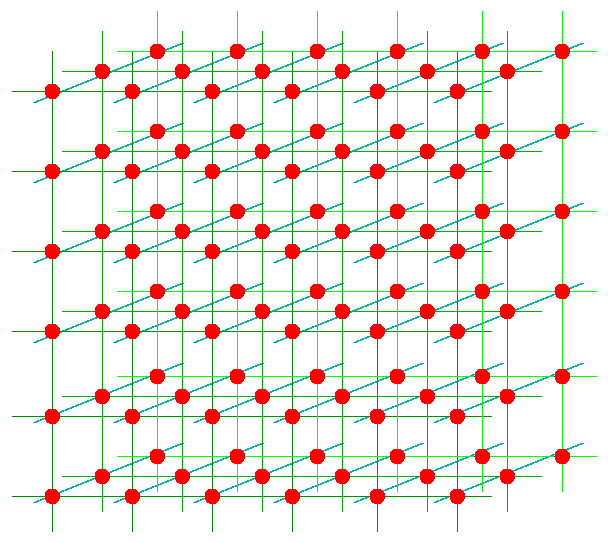
\includegraphics[width=3.0in]{lattice.png}\hspace*{8mm}
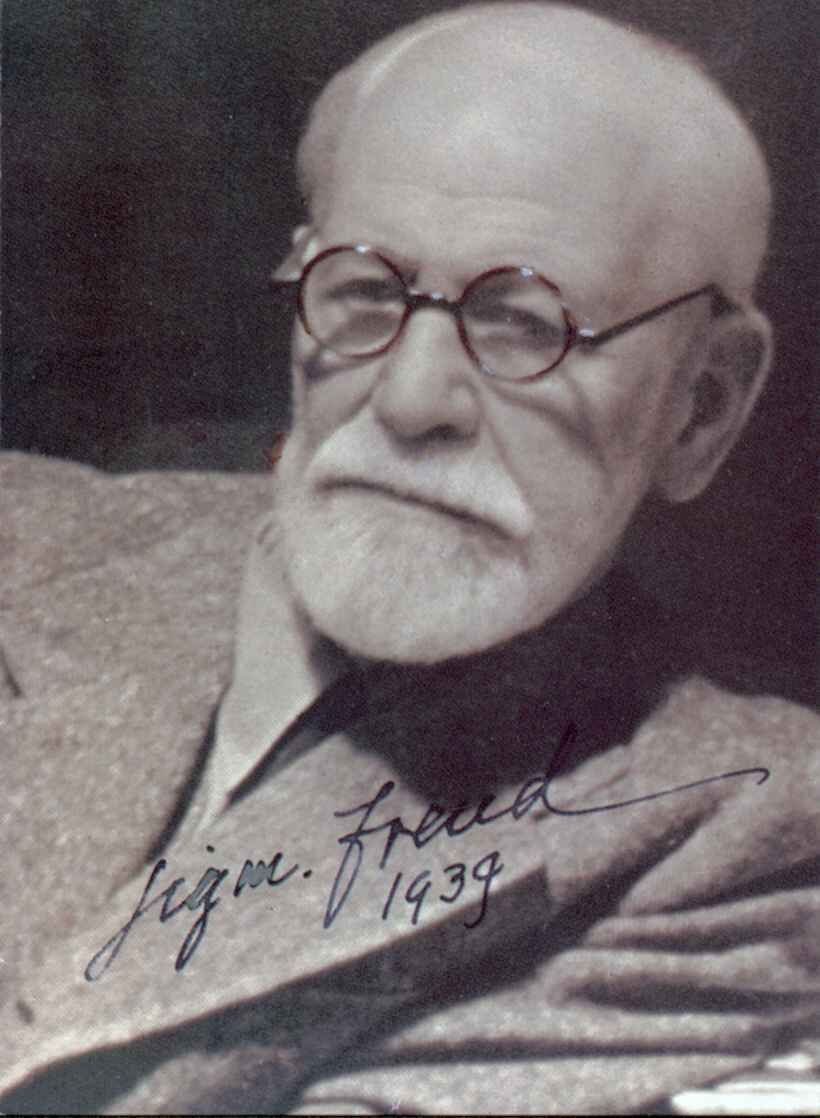
\includegraphics[width=2.0in]{freud.jpg}
\end{center}

\newpage

\tableofcontents

\newpage

\section{Introduction}

\sigmond is a software suite for the analysis of Monte Carlo data in
lattice QCD.  The name \texttt{sigmond} comes from \underline{sig}nal
extraction from \underline{Mon}te Carlo \underline{d}ata, and also plays
upon the name ``Sigmund'' from Sigmund Freud, a neurologist famous for
his analytical thinking.
\sigmond currently runs only in batch mode.
%\sigmond runs in three modes: batch,
%command-line-interface (CLI) interactive, and
%graphical-user-interface (GUI) interactive.
We assume \sigmond is being used
in a linux environment.  These notes focus on the use of the software,
so little is said here about how to compile the software.\\

The source software, build directories with make files, and documentation
are bundled in the compressed tar file \vb{sigmond.tar.gz}.  Issue the
command
\begin{verbatim}
    tar xzvf sigmond.tar.gz
\end{verbatim}
which creates a single directory \vb{sigmond} in the current directory.
\vb{cd} into this directory, and one sees subdirectories named \vb{source},
\vb{build}, and \vb{doc}.  This user guide (LaTeX and pdf files)
is stored in the \vb{doc} subdirectory.  All source files are contained in
the \vb{source} directory.   Before compiling, be sure to edit the file
\vb{sigmond/build/Makefile.inc}.  To compile \vb{sigmond} in batch mode,
\vb{cd} into the \vb{build/batch} directory and
issue a \vb{make} command. \\
%To compile the CLI version, \vb{cd} into the
%\vb{build/cli} directory and issue a \vb{make} command, whereas to compile
%the GUI version, \vb{cd} into the \vb{build/gui} directory and
%issue a \vb{make} command.

Other libraries which are necessary include \vb{lapack}, \vb{xmgrace} (plotter),
and \vb{Minuit2}.
%and \vb{gtkmm3} (for the graphical user interface).
Edit the file
\vb{sigmond/build/Makefile.inc} to specify the location of the needed
libraries and header files on your system.  You should change the \vb{SRC\_DIR}
entry in this file to the full path name of the directory on your system
where you untarred the \vb{sigmond} directory.\\

In batch mode, a single input file must be given as a command line
argument.  The input file must contain an XML document which
tells \sigmond what data to analyze and what tasks to do.  The structure
and allowed content of the XML input is the subject of these notes and
is described in detail below.  If the input XML file is named
\vb{input.xml}, then a batch run is accomplished by the command
\begin{verbatim}
    sigmond_batch input.xml
\end{verbatim}

%In interactive mode, the command line argument specifying an XML
%input document is optional.  Interactive mode is trivial to use
%once batch mode is understood, so these notes focus on the batch mode
%of \vb{sigmond}.

\vb{sigmond} writes and reads binary data files.  It can write out
both bin and sampling files.  A bin file contains Monte Carlo data
of so-called simple observables corresponding to an integrand in a Monte
Carlo integrand, something that can be defined on a single field
configuration.  Several of such successive measurements can be averaged
into a so-called bin, and the file stores these bins for subsequent
reading and analysis.  Sampling files contain resampling values using
either jackknife or bootstrap resampling.  Other various files can
be written and read, such as those containing information about
correlation matrix rotations and transformations.  Any file format
written by \vb{sigmond} can, of course, be read by \vb{sigmond}.
Currently, \vb{sigmond} can read files in the format created by
\vb{chroma\_laph} and \vb{last\_laph}.  Of course, \vb{sigmond} can be
re-programmed to utilize other data formats by changing the source files
in the \vb{source/data\_handling} subdirectory. \vb{sigmond} also writes
log files in XML format, as well as \vb{xmgrace} files for plots.
More on file formats is discussed later in these notes.

\section{Overview of the XML input}
The input XML document must have a root tag named \vb{<SigMonD>}.
Inside this root tag, there must be one tag named \vb{<Initialize>},
and another tag named \vb{<TaskSequence>}.  Specification of the data
files, the log file, and so on, must be located in the \vb{<Initialize>}
tag.  The tasks to be performed using the data are then placed inside
the \vb{<TaskSequence>} tag.   The input XML file must have the form
given below.

\begin{verbatim}
<SigMonD>

    <Initialize>
        <ProjectName> Name Of Project </ProjectName>
        <LogFile> log_output.xml </LogFile>
        <KnownEnsemblesFile>/path/ensembles.xml</KnownEnsemblesFile> (optional)
        <EchoXML/>  (optional)
        <MCBinsInfo>  ...  </MCBinsInfo>
        <MCSamplingInfo> ... </MCSamplingInfo>
        <MCObservables>  ...  </MCObservables>
    </Initialize>

    <TaskSequence>
        <Task><Action>...</Action> ... </Task>
        <Task><Action>...</Action> ... </Task>
        ....
    </TaskSequence>

</SigMonD>
\end{verbatim}

\section{The data initializer tag}
The \vb{<Initialize>} tag must contain the data files, the log file, and so on.
This tag must have the form:
\begin{verbatim}
<Initialize>
    <ProjectName> Name Of Project </ProjectName>
    <LogFile> log_output.xml </LogFile>
    <KnownEnsemblesFile>/path/ensembles.xml</KnownEnsemblesFile>
    <EchoXML/>
    <MCBinsInfo>  ...  </MCBinsInfo>
    <MCSamplingInfo> ... </MCSamplingInfo>
    <MCObservables>  ...  </MCObservables>
</Initialize>
\end{verbatim}
\begin{itemize}
\item
  If \vb{<ProjectName>} is missing, a default name will be created.
\item
  If \vb{<LogFile>} is missing, a default name for the log file is used.
  Output to this file will be in XML format.
\item
  The tag \vb{<KnownEnsemblesFile>} is optional and is described below.
\item
  If \vb{<EchoXML/>} is missing, the input XML will not be written (echoed)
  to the log file.
\item
  The tag \vb{<MCBinsInfo>} is mandatory: it specifies the ensemble,
  controls rebinning the data, and possibly omitting certain configurations
  in the ensemble if these is data corruption.  This tag is described below.
\item
  The tag \vb{<MCSamplingInfo>} is mandatory.  It controls the default
  resampling method:  jackknife or bootstrap.  This default method
  is assumed for all reading and writing sampling results to and
  from files.  Note that both jackknife and bootstrap resampling
  can be done in any program execution, but only one can be used
  for reading/writing to files.  A more detailed
  description of this tag is given below.
\item
  \vb{<MCObservables>} describes the data to be input for analysis. This
  tag is described in detail below.
\end{itemize}

\subsection{The known ensembles information file}
Various Monte Carlo ensembles are made known to \vb{sigmond} in the 
ensembles XML file so that one only need specify an identification
string to \vb{sigmond} and \vb{sigmond} will know all that it needs to
know about the ensemble.  The absolute path to this file can be specified in
the \vb{<KnownEnsemblesFile>} tag.  If not given, a default location
for this file has been stored during the compilation.  This file must have 
information specified in the following XML format:
\begin{verbatim}
   <KnownEnsembles>
     <Infos>
       <EnsembleInfo>...</EnsembleInfo>
       <EnsembleInfo>...</EnsembleInfo>
        ....
     </Infos>
     <CLSEnsembleWeights>
       <Ensemble>...</Ensemble>
        ....
     </CLSEnsembleWeights>
   </KnownEnsembles>
\end{verbatim}
with each ensemble in the \vb{<Infos>} tags specified by
\begin{verbatim}
   <EnsembleInfo>
      <Id>clover_s24_t128_ud840_s743</Id>
      <NStreams>4</NStreams>
      <NMeas>551</NMeas>
      <NSpace>24</NSpace>
      <NTime>128</NTime>
      <Weighted/>  (if has CLS weights; omit otherwise)
   </EnsembleInfo>
\end{verbatim}
The entries in the \vb{<CLSEnsembleWeights>} tag must have the form:
\begin{verbatim}
   <Ensemble>
      <Id>cls21_D200_r000</Id>
      <Weights> 0.999 0.998 ... </Weights>
   </Ensemble>
\end{verbatim}

\subsection{The bins information tag}

The tag \vb{<MCBinsInfo>} is mandatory: it identifies the Monte Carlo
ensemble and controls rebinning the data,
and possibly omitting certain configurations in the ensemble (for example,
if certain measurements have been corrupted).  The XML must have the form
below:
\begin{verbatim}
<MCBinsInfo>
  <MCEnsembleInfo>clover_s24_t128_ud840_s743</MCEnsembleInfo>
  <TweakEnsemble>
     <Rebin>2</Rebin>
     <Omissions>2 7 11</Omissions>
  </TweakEnsemble>
</MCBinsInfo>
\end{verbatim}
The tag \vb{<MCEnsembleInfo>} tag is mandatory and identifies the
ensemble of configurations upon which all calculations are based.
The string inside this tag must match one of the ensemble identification
strings known to \vb{sigmond}.  Known ensembles are stored in a file,
usually named \texttt{ensembles.xml}, which was discussed above.  
Given one of the identifying strings specified in the file \texttt{ensembles.xml}, 
\vb{sigmond} class knows how many
Markov-chain streams are available, how many RHMC trajectory numbers are
valid, and so on.

If you are using only a small fraction of the configurations, it is 
easier to use
\begin{verbatim}                                                    
  <TweakEnsemble>                                                 
    <KeepFirst>3</KeepFirst>  (index of first config to keep)     
    <KeepLast>12</KeepLast>   (index of last config to keep)      
  </TweakEnsemble>                                                   
\end{verbatim}

To specify an ensemble not known to SigMonD, you must provide
the following information:
$\{n_{\rm meas}, \; n_{\rm streams}, \; n_x, \; n_y, \; n_z, \; n_t\}$
This is done by appending to the id string fields that give
this information in the order above, separated by ``\vb{|}''.
Example:
\begin{verbatim}
   <MCEnsembleInfo>idname|800|1|24|24|24|36</MCEnsembleInfo>
\end{verbatim}

The \vb{<TweakEnsemble>} tag is optional.
In the \vb{<Rebin>} tag, a positive integer should be given.  That number of
successive Monte Carlo measurements are combined into a single bin.
If there are $N$ measurements, and \vb{<Rebin>} is input as $n$,
there will be $N/n$ bins. The \vb{<Omissions>} tag, if present,
should contain non-negative integers corresponding to the configurations
(measurements) to omit. These indices are zero offset, that is, the
first configuration in the ensemble is numbered zero.

\subsection{The default sampling information tag}
The tag \vb{<MCSamplingInfo>} is mandatory.  It controls the default
resampling method:  jackknife or bootstrap.  This default method
is assumed for all reading and writing sampling results to and
from files.  Note that both jackknife and bootstrap resampling
can be done in any program execution, but only the default method can be used
for reading/writing to files.  For specifying jackknife resampling as
the default, the XML input must have the form
\begin{verbatim}
<MCSamplingInfo>
   <Jackknife/>
</MCSamplingInfo>
\end{verbatim}
To specify bootstrap resampling as the default, the XML input must have the
form below, which provides details about the bootstrapping:
\begin{verbatim}
<MCSamplingInfo>
   <Bootstrapper>
      <NumberResamplings>2048</NumberResamplings>
      <Seed>6754</Seed>
      <BootSkip>127</BootSkip>
      <Precompute/>
   </Bootstrapper>
</MCSamplingInfo>
\end{verbatim}
\vb{<Seed>} must be an unsigned 32-bit integer $0\ \dots\ 2^{32}-1$.
For a given bootstrap resampling, the Mersenne twister is
called in sequence to generate the sample. Before generating
the next resampling, the Mersenne twister is called \vb{<BootSkip>}
number of times. The \vb{<BootSkip>} parameter allows more variety
in how the bootstrap resamplings are generated. If the \vb{<Precompute>}
empty tag is present, then the bootstrap indices are computed all at once
and stored in memory. If not present, the bootstrap indices are computed
``on the fly''. The bootstrap samples are generated using the Mersenne
twister, but in a pseudorandom way that is repeatable. So a given resampling
can be regenerated as needed. Including \vb{<Precompute>} uses more memory.
Try your computations with and without this tag to see which is faster,
since speed depends on memory access speed.

\subsection{The observables tag}
The \vb{MCObservables} tag specifies the data files to use in looking
for the necessary Monte Carlo measurements, as well as the observables
themselves, optionally.  This tag must have the form:
\begin{verbatim}
<MCObservables>
    <BLCorrelatorData>            <-- basic LapH correlator data files
        <FileListInfo>...</FileListInfo>
        <FileListInfo>...</FileListInfo>
           ....
    </BLCorrelatorData>
    <BLVEVData>                   <-- basic LapH VEV data files
        <FileListInfo>...</FileListInfo>
        <FileListInfo>...</FileListInfo>
           ....
    </BLVEVData>
    <BinData>                     <-- bin files in sigmond format
        <FileName>...</FileName>
         ....
    </BinData>
    <SamplingData>                <-- resampling files in sigmond format
        <FileName>...</FileName>
         ....
    </SamplingData>
    <UseCheckSums/>  (optional)
    <Specifications>
          ...
        specifications of observables (optional)
          ...
    </Specifications>
</MCObservables>
\end{verbatim}

Files containing basic LapH (see later) data for the temporal correlators to be analyzed
must be specified in terms of \vb{<FileListInfo>} tags inside a
\vb{<BLCorrelatorData>} tag.  Similarly, files containing basic LapH data for
any vacuum expectation values must be specified in terms
of \vb{<FileListInfo>} tags inside a \vb{<BLVEVData>} tag.  Bin files
in \vb{sigmond} format must be specified in a \vb{<BinData>} tag, and sampling files
in \vb{sigmond} format must be listed in a \vb{<SamplingData>} tag.

Each \vb{<FileListInfo>} tag must have the form
\begin{verbatim}
<FileListInfo>
    <FileNameStub>  ...  </FileNameStub>
    <MinFileNumber> ...  </MinFileNumber> (default=0)
    <MaxFileNumber> ...  </MaxFileNumber>
    <FileMode>      ...  </FileMode>      (optional)
</FileListInfo>
\end{verbatim}
Each \vb{<FileListInfo>} tag contains information about a list of files
having a common stub and a numerical suffix from a minimum value to a
maximum value. For example, if \vb{<FileNameStub>} contained
\vb{/data/correlators/corr}, \vb{<MinFileNumber>} contained
\vb{10}, and \vb{<MaxFileNumber>} contained \vb{12}, then
the three files named \vb{corr.10}, \vb{corr.11}, and \vb{corr.12}
in the directory \vb{/data/correlators} would be read by \vb{sigmond}.
The \vb{<FileMode>} tag is provided to indicate whether
files may be overwritten. To allow for overwriting, the
\vb{<FileMode>} tag must contain the word \vb{overwrite}. Otherwise,
files will be protected from possible overwriting.

Observables can be specified inside a \vb{<Specifications>} tag.  If no
observables are specified, then all observables found while reading the
files will be used.  If any observables \textit{are} specified, then only
those observables will be considered for input: files corresponding to other
observables will be ignored, and an exception is thrown if the file
containing the data for any requested observable cannot be found.

Observables can be specified inside a \vb{<Specifications>} tag as follows:
\begin{description}
\item[(a)]
  a single correlator (no VEV subtraction)
\begin{verbatim}
<Correlator>
  <Source><Operator>...</Operator></Source>
  <Sink><Operator>...</Operator></Sink>
</Correlator>
\end{verbatim}
\item[(b)]
  a single correlator with VEV subtraction
\begin{verbatim}
<CorrelatorWithVEV>
  <Source><Operator>...</Operator></Source>
  <Sink><Operator>...</Operator></Sink>
</CorrelatorWithVEV>
\end{verbatim}
\item[(c)]
  a single VEV
\begin{verbatim}
<VEV><Operator>...</Operator></VEV>
\end{verbatim}
\item[(d)]
  a Hermitian matrix of correlators (no VEV subtraction)
\begin{verbatim}
<HermitianCorrelationMatrix>
  <Operator>...</Operator>
  <Operator>...</Operator>
         ...
</HermitianCorrelationMatrix>
\end{verbatim}
\item[(e)]
  a Hermitian matrix of correlators with VEV subtraction
\begin{verbatim}
<HermitianCorrelationMatrixWithVEVs>
  <Operator>...</Operator>
  <Operator>...</Operator>
       ...
</HermitianCorrelationMatrixWithVEVs>
\end{verbatim}
\item[(f)]
  matrix of correlators (no Hermiticity, no VEV subtract)
\begin{verbatim}
<CorrelationMatrix>
  <Operator>...</Operator>
  <Operator>...</Operator>
       ...
</CorrelationMatrix>
\end{verbatim}
\item[(g)]
  matrix of correlators with VEV subtract (no Hermiticity)
\begin{verbatim}
<CorrelationMatrixWithVEVs>
  <Operator>...</Operator>
  <Operator>...</Operator>
        ...
</CorrelationMatrixWithVEVs>
\end{verbatim}
\item[(h)]
  set of observables in bin files (non basic LapH) of \vb{sigmond} format
\begin{verbatim}
<ObsBins>
  <MCObservable>...</MCObservable>
  <MCObservable>...</MCObservable>
         ...
</ObsBins>
\end{verbatim}
\item[(i)]
  set of observables in sampling files of \vb{sigmond} format
\begin{verbatim}
<ObsSamplings>
  <MCObservable>...</MCObservable>
  <MCObservable>...</MCObservable>
        ...
</ObsSamplings>
\end{verbatim}
\end{description}

Details concerning how to specify a QCD operator in an \vb{<Operator>}
tag and all observables in an \vb{<MCObservable>} tag are described in the
next section.  In all of the above tags, the alternative tags \vb{<BLOperator>},
\vb{<GIOperator>}, \vb{<OperatorString>}, \vb{<BLOperatorString>}, and
\vb{<GIOperatorString>} can be used wherever an \vb{<Operator>} is used.
These tags are explained in the next section.
If a tag \vb{<AllHermitian/>} appears inside the \vb{<Specifications>}
tag, then all correlation matrices are treated as Hermitian.

\section{Monte Carlo observables and operators}

A key concept used by \vb{sigmond} is that of a Monte Carlo observable.
Each observable must be associated with a \textit{real-valued} quantity that
can be estimated by our Monte Carlo path integrals.  These can be simple
quantities, such as the real or imaginary part of a temporal correlator for
one time separation, that can be defined on a single gauge configuration,
or much more complicated quantities, such as a fit parameter yielding a
stationary-state energy, determined by fitting a decaying exponential to a
temporal correlation function.

Many Monte Carlo observables involve quantum field operators.  For example,
the real and the imaginary parts of the vacuum expectation value of a QCD
field operator are examples of Monte Carlo observables here.  The real
and the imaginary parts of the temporal correlation of two operators
separated by some time interval are also Monte Carlo observables.  So
defining and specifying QCD operators is an important part of specifying
Monte Carlo observables.  In this section, a variety of operators are
first discussed, and then the all-important \vb{<MCObservable>} tag is
discussed.

\subsection{Basic LapH operators}
\label{sec:qcd_op_tag}
A so-called \textit{basic LapH} QCD operator can be specified in ``long form''
by an \vb{<Operator>} or \vb{<BLOperator>} tag,
or in ``short form'' by an \vb{<OperatorString>} or \vb{<BLOperatorString>} tag.
A basic LapH operator is an assemblage of covariantly-displaced LapH-smeared
quark fields in a variety of spatial orientations.
The XML format for specifying an operator must be of the form:
\begin{verbatim}
<BLOperator>
    <NumberOfHadrons> 2 </NumberOfHadrons>
        ....
</BLOperator>
\end{verbatim}
or of the form (see below)
\begin{verbatim}
    <BLOperatorString> ... </BLOperatorString>
\end{verbatim}
An \vb{<BLOperator>} tag must contain a \vb{<NumberOfHadrons>} tag.
The rest of the XML depends on the number of hadrons.
A ``hadron'' here means a baryon, a meson, or a glueball.
It could also mean a tetraquark system, a pentaquark system,
\textit{etc.}  It is a gauge-invariant localized quantity.
\begin{itemize}
\item
  Number of hadrons = 0:
  No further tags are required
  (this is the ``default'' constructor).
\item
  Number of hadrons = 1: XML must include
\begin{verbatim}
<Hadron>
   ....described below....
</Hadron>
<LGIrrepRow> 3 </LGIrrepRow>
\end{verbatim}
\item
  Number of hadrons = 2,\ 3,\ 4,\dots:  XML must include
\begin{verbatim}
<Total>
   <Isospin> triplet </Isospin>
   <IsoCGId> 0 </IsoCGId>} (assume zero if absent)
   <Momentum>  0 0 0  </Momentum>
   <LGIrrep> T1gm </LGIrrep>
   <LGCGId> 0 </LGCGId>} (assume zero if absent)
   <LGIrrepRow> 3 </LGIrrepRow>
</Total>
<Hadron1>
    ....
</Hadron1>
<Hadron2>
    ....
</Hadron2>
   ....
\end{verbatim}
\end{itemize}
In the \vb{<Total>} tag, the \vb{<Isospin>} tag must take a value such
as \vb{singlet}, \vb{doublet}, \vb{triplet}, \textit{etc.}  When there are
three or more hadrons, an isospin Clebsch-Gordan occurrence
identifying number must be specified in a \vb{IsoCGId} tag: value 0 to
one less than the number of times that the irrep specified in the
\vb{<Isospin>}
tag occurs in
the direct product of the single-hadron isospins.  A value
of zero for this tag is assumed if the tag is absent.
If the irrep occurs more than once in the Clebsch-Gordan
series of the direct product of single-hadron irreps, then
a little group Clebsch-Gordan identifying number
must be specified (value 0 to one less than the number of
occurrences) in a \vb{<LGCGId>} tag.  A value of 0 is assumed if absent.

The constituent single-hadron operators inside an \vb{<BLOperator>} tag
must be described in
separate tags named \vb{<Hadron1>}, \vb{<Hadron2>}, \textit{etc.}  If a single hadron
is a meson or a baryon, then a single \vb{<Hadron>} tag must occur.
Single hadron tags must have the form
\begin{verbatim}
<Hadron1>
    <Flavor> eta </Flavor>
    <Momentum>  0 0 0  </Momentum>
    <LGIrrep> A1p </LGIrrep>
    <SpatialType> DDL </SpatialType>
    <SpatialIdNum> 4 </SpatialIdNum>
    <DispLength> 3 </DispLength>
</Hadron1>
\end{verbatim}
Allowed meson \vb{<Flavor>} tag values are \vb{pion}, \vb{eta}, \vb{phi},
\vb{kaon}, and \vb{kbar}. Note that \vb{pion} does \textit{not} mean an actual
pion, rather, it just means an isovector consisting of $u,d$
quarks.  \vb{pion} is just a shorter name than \vb{isovector\_du}.
Similarly, an \vb{eta} means an isoscalar meson consisting of
$\overline{u}u+\overline{d}d$ quarks.  A \vb{phi} is an isoscalar meson
that is $\overline{s}s$.
\vb{kaon} refers to a strangeness $S=1$ meson, and \vb{kbar} refers
to a strangeness $S=-1$ meson. Allowed baryon \vb{<Flavor>} tag
values are \vb{nucleon}, \vb{delta}, \vb{lambda}, \vb{sigma}, \vb{xi}, and
\vb{omega}.  \vb{<Momentum>} is the momentum of the particle
in a chosen ``reference'' term of the total operator.  The
total momentum can be obtained by adding all of the single
hadron momenta, and the total momentum is fixed.  The total
operator is a superposition of terms that are rotations,
parity-transformations, and $G$-parity transformations of the
reference term. Each \vb{<Momentum>} tag must contain three
integers (in units of $2\pi/L$, where $L$ is the spatial extent of the
$L^3$ lattice volume) which describe the momentum
of the hadron in the reference term. \vb{<LGIrrep>} specifies the
irreducible representation of the little group corresponding
to the hadron momentum.

If the single constituent is a glueball, then its \vb{<Hadron>}
tag must be of the form
\begin{verbatim}
<Hadron1>
    <Flavor> glueball </Flavor>
    <Momentum>  0 0 0  </Momentum>
    <LGIrrep> A1gp </LGIrrep>
    <SpatialType> TrEig </SpatialType>
</Hadron1>
\end{verbatim}

If the single constituent is a tetraquark, then its \vb{<Hadron>}
tag must be of the form
\begin{verbatim}
<Hadron1>
   <Flavor> isotriplet_phi_pion </Flavor>
   <Momentum>  0 0 0  </Momentum>
   <LGIrrep> A1gm </LGIrrep>
   <SpatialType> QDX </SpatialType>
   <SpatialIdNum> 2 </SpatialIdNum>
   <DispLength> 3 </DispLength>
   <ColorType> 1 </ColorType>  (or -1)
</Hadron1>
\end{verbatim}
Allowed tetraquark \vb{<Flavor>} tag values are shown in
the first column of the table below.  When using the
short hand \vb{<BLOperatorString>} form (see below),
tetraquarks are specified using the short notation in
the second column below.  The final \vb{p} in the
entries of the second column refers to color symmetric.
For color antisymmetric operators, replace the \vb{p}
by \vb{m}.
\begin{center}\renewcommand{\arraystretch}{1.0}
\begin{tabular}{lc}
 &                        (short notation)\\
\vb{isosinglet\_eta\_eta}   & \vb{tquuuu1p}\\
\vb{isotriplet\_eta\_pion}  & \vb{tquudu3p}\\
\vb{isosinglet\_pion\_pion} & \vb{tqdudu1p}\\
\vb{isotriplet\_pion\_pion} & \vb{tqdudu3p}\\
\vb{isoquintet\_pion\_pion} & \vb{tqdudu5p}\\
\vb{isodoublet\_kaon\_eta}  & \vb{tqsuuu2p}\\
\vb{isodoublet\_kaon\_pion} & \vb{tqsudu2p}\\
\vb{isoquartet\_kaon\_pion} & \vb{tqsudu4p}\\
\vb{isotriplet\_phi\_pion}  & \vb{tqssdu3p}\\
\vb{isosinglet\_eta\_phi}   & \vb{tquuss1p}\\
\vb{isodoublet\_kaon\_phi}  & \vb{tqsuss2p}\\
\vb{isosinglet\_phi\_phi}   & \vb{tqssss1p}
\end{tabular}
\end{center}

An operator can also be specified by a short string inside an
\vb{<BLOperatorString>} tag.  For example:
\begin{verbatim}
<BLOperatorString> glueball P=(0,0,0) A1gp_1 TrEig </BLOperatorString>
<BLOperatorString> pion P=(0,0,0) A1um_1 SD_5  </BLOperatorString>
<BLOperatorString> isotriplet_pion_pion A1um_1 CG_1 [P=(0,0,1) A1p LSD_1]
  [P=(0,0,-1) A2m TSD_2] </BLOperatorString>
<BLOperatorString> tquuuu1p P=(0,0,0) A1um_1 QDX_1</BLOperatorString>
\end{verbatim}
If the \vb{CG\_1} token is absent, a value 0 is assumed.
If the displacement length is omitted, then default values are used: 
3 for mesons, 2 for tetraquarks and baryons.

\subsection{General irreducible operators}

Other QCD operators are called general irreducible operators
and are specified inside a \vb{<GIOperator>} tag. For example,
a ``rotated'' operator or other linear superpositions of the
basic operators are general irreducible operators.  The XML
format for specifying such an operator must be of the form
\begin{verbatim}
<GIOperator>
   <Isospin> triplet </Isospin>
   <Momentum>  0 0 0  </Momentum>
      or <MomentumSquared> 0 </MomentumSquared>
   <LGIrrep> T1gm </LGIrrep>
   <LGIrrepRow> 3 </LGIrrepRow>
   <IDName>a_string_no_whitespace</IDName> (24 char max)
   <IDIndex> 0 </IDIndex> (0 if absent)
</GIOperator>
\end{verbatim}
or using the shorter form
\begin{verbatim}
<GIOperatorString>isotriplet P=(0,0,0) A1um_1 IDname 2</GIOperatorString>
\end{verbatim}
The \vb{<IDName>} tag content must be a string containing no white space
and no more than 24 characters in length.  The \vb{<Isospin>} tag must take 
a value such as \vb{singlet}, \vb{doublet}, \vb{triplet}, and so on.

You can also specify the momentum squared and/or leave out the irrep row 
(\textit{e.g.,} if it was averaged over).  For example,
\begin{verbatim}
  <GIOperatorString>isotriplet S=-1 PSQ=1 A2m IDname 2</GIOperatorString>
\end{verbatim}
If the \vb{IDIndex} token is absent, a value 0 is assumed.

\subsection{Temporal correlators}

Information about a temporal correlator can be specified with a
\vb{<Correlator>} tag using XML of the form
\begin{verbatim}
<Correlator>
   <Source><Operator>..</Operator></Source>
   <Sink><Operator>..</Operator></Sink>
</Correlator>
\end{verbatim}
Inside the \vb{<Source>} and \vb{<Sink>} tags, one can use one of
the following tag types:
\vb{<Operator>}, \vb{<BLOperator>}, \vb{<GIOperator>}, or the shorter
\vb{<OperatorString>}, \vb{<BLOperatorString>}, or
\vb{<GIOperatorString>} tags.

A temporal correlator at one particular time separation is specified
by XML of the form
\begin{verbatim}
<Correlator>
   <Source><Operator>..</Operator></Source>
   <Sink><Operator>..</Operator></Sink>
   <TimeIndex>..</TimeIndex>
   <HermitianMatrix/>             (optional)
   <SubtractVEV/>                 (optional)
</Correlator>
\end{verbatim}
where the \vb{<TimeIndex>} specifies the requested time separation.
If the \vb{<HermitianMatrix>} tag is given, this facilitates
input which automatically averages using the complex conjugate
elements, if available.  VEV subtraction is specified by the
\vb{<SubtractVEV/>} tag.

\subsubsection{\vb{CorrelatorMatrixInfo}}
We may also specify a more general temporal correlation matrix,
including whether VEV subtraction is needed and if the matrix is
hermitian or not. The XML must be of the form
\begin{verbatim}
<CorrelatorMatrixInfo>
    <Operator>...</Operator>
    <Operator>...</Operator>
 (or   <OperatorString>...</OperatorString>)
         ...
    <HermitianMatrix/>    (optional)
    <SubtractVEV/>    (optional)
    <AssignName>descriptive_name</AssignName>
</CorrelatorMatrixInfo>
\end{verbatim}
or recalled by
\begin{verbatim}
<CorrelatorMatrixInfo>
    <Name>descriptive_name</Name>
</CorrelatorMatrixInfo>
\end{verbatim}

\subsubsection{\vb{DiagonalCorrelatorSet}} \label{sec:diag_corr_set}
\sigmond provides a class that is useful for storing information
about a diagonal set of correlators. The CorrelatorInfo is
available for each entry as well as information related to a fit
to each correlator. The XML construction can take different forms,
either with the \vb{<Sequential>} tag to specify the listed
operators in an explicit ordering or with \newline\vb{<OperatorIndex>}
tags to give the operator orderings. Valid input XML can look like

\begin{description}
\item[(a)]
\begin{verbatim}
<DiagonalCorrelatorSet>
   <DiagonalCorrelator>
      <OperatorString>pion P=(0,0,0) A1um_1 SS_0</OperatorString>
      <OperatorIndex>0</OperatorIndex>
   </DiagonalCorrelator>
   <DiagonalCorrelator>
      <OperatorString>kaon P=(0,0,0) A1u_1 SS_0</OperatorString>
      <OperatorIndex>1</OperatorIndex>
   </DiagonalCorrelator>
   <SubtractVEV/>   (optional)
</DiagonalCorrelatorSet>
\end{verbatim}
or
\item[(b)]
\begin{verbatim}
<DiagonalCorrelatorSet>
  <Sequential>
      <OperatorString>pion P=(0,0,0) A1um_1 SS_0</OperatorString>
      <OperatorString>kaon P=(0,0,0) A1u_1 SS_0</OperatorString>
  </Sequential>
   <SubtractVEV/>   (optional)
</DiagonalCorrelatorSet>
\end{verbatim}
or
\item[(c)] from a rotated correlation matrix (\ref{sec:rotation})
\begin{verbatim}
<DiagonalCorrelatorSet>
  <RotatedSequential>
     <GIOperatorString>....</GIOperatorString> (can omit ID index)
     <NumberOfLevels>34</NumberOfLevels>
  </RotatedSequential>
  <SubtractVEV/>   (optional)
</DiagonalCorrelatorSet>
\end{verbatim}
or
\item[(d)] from a general correlation matrix
\begin{verbatim}
<DiagonalCorrelatorSet>
  <CorrelatorMatrixInfo>
  ....
  </CorrelatorMatrixInfo>
</DiagonalCorrelatorSet>
\end{verbatim}
\end{description}

\subsection{Monte Carlo observables} \label{sec:mcobs}

The all-important \vb{<MCObservable>} tag is used to specify one particular
Monte Carlo observable. This will be used extensively in many
of the tasks, which will be introduced later in these notes.
Each observable must be associated with a \textit{real-valued}
quantity that can be estimated by our Monte Carlo path integrals.
These can be simple quantities, such as the real or imaginary part of
a temporal correlator for one time separation, that can be
defined on a single gauge configuration, or much more
complicated quantities, such as a fit parameter yielding a
stationary-state energy, determined by fitting a decaying
exponential to a temporal correlation function.\\

An observable is termed \textit{simple} if it can be associated with
the integrand of a single path integral.  Simple observables include
the real or imaginary part of a temporal correlator
for one time separation, and the real or imaginary part of a vacuum
expectation value.  Other observables are referred to as \textit{nonsimple}.\\

The \vb{<MCObservable>} tag is meant to encompass all observables
of interest.  Observables can be classified as \textit{primary} or
\textit{secondary}:  ``primary'' refers to operator VEVs and correlators of
field operators, which can be of type ``BasicLapH'' or ``GenIrrep'', and
``secondary'' refers to fit parameters and other user-defined
observables.\\

There are two types of primary observables currently implemented: vacuum
expectation values of an operator, and temporal correlators of two
operators for one time separation.  A VEV is specified by the following XML:
\begin{verbatim}
<MCObservable>
   <VEV><Operator>..</Operator></VEV>
   <Arg>RealPart</Arg>
</MCObservable>
\end{verbatim}
In the \vb{<Arg>} tag, the content can be either \vb{Re},
\vb{RealPart}, \vb{Im}, or \vb{ImaginaryPart}.
A correlator at a particular time separation is specified by XML for the form
\begin{verbatim}
<MCObservable>
   <Correlator>
      <Source><Operator>..</Operator></Source>
      <Sink><Operator>..</Operator></Sink>
      <TimeIndex>..</TimeIndex>
      <HermitianMatrix/>    (optional)
      <SubtractVEV/>    (optional)
   </Correlator>
   <Arg>RealPart</Arg>
</MCObservable>
\end{verbatim}
Again, in the above,  \vb{<BLOperator>}, \vb{<GIOperator>}, or the shorter
\vb{<OperatorString>}, \vb{<BLOperatorString>}, or
\vb{<GIOperatorString>} tags can be used wherever an \vb{<Operator>}
tag is used. If the \vb{<HermitianMatrix/>} tag is given, this facilitates
input which automatically averages using the complex
conjugate elements, if available.  If \vb{<Arg>} is omitted, then
the real part is assumed.\\

Secondary observables are specified using a \vb{<ObsName>} tag and
an unsigned integer \vb{<Index>} tag.  An optional \vb{<Arg>} tag
(assumed RealPart if absent) and an optional \vb{<Simple/>}
tag (if absent, the observable is assumed to be nonsimple) can also
be included.   In summary, the XML for a secondary operator takes the form
\begin{verbatim}
<MCObservable>
   <ObsName>T1upEnergy</ObsName>      (32 char or less, no white space)
   <Index>3</Index>                   (opt nonneg integer: default 0)
   <Simple/>                          (if simple observable)
   <Arg>RealPart</Arg>
</MCObservable>
\end{verbatim}

\section{File formats}

\vb{sigmond} assumes the Monte Carlo data files are in the format
created by \vb{chroma\_laph} and \vb{last\_laph}, which use objects
of a templated class named \vb{IOMap<K,V>}, where \vb{K} is a record
key type and \vb{V} is a data type, to write the data to various
files.  Each file created by \vb{IOMap} contains in the following order:\\
\hspace*{20pt}(1) a character `L' or `B' indicating endianness\\
\hspace*{20pt}(2) a 32-character ID string\\
\hspace*{20pt}(3) address offset location where the map is stored in the file (8 bytes) \\
\hspace*{20pt}(4) a character `Y' or `N' describing if checksums are stored in the file \\
\hspace*{20pt}(5) a header string of any length\\
\hspace*{20pt}(6) the data records one after another \\
\hspace*{20pt}(7) the file map containing the keys and the offset locations of the records\\
\hspace*{20pt}(8) an ending character `E'\\
Each record contains in the following order:\\
\hspace*{20pt}(1) the size in bytes of the record (excluding checksum)\\
\hspace*{20pt}(2) the data itself in binary format\\
\hspace*{20pt}(3) the checksum of the data (optionally).\\
Of course, \vb{sigmond} can be re-programmed to utilize other data formats
by changing the source files in the \vb{source/data\_handling} subdirectory.


\section{The task sequence tag}

The \vb{<TaskSequence>} tag specifies the tasks to be performed using the
Monte Carlo data.  This tag is needed in batch mode, but
can be omitted in interactive mode.  If present, this tag must have the form:
\begin{verbatim}
<TaskSequence>
    <Task><Action>...</Action> ...  </Task>
    <Task><Action>...</Action> ...  </Task>
     ....
</TaskSequence>
\end{verbatim}
Each \vb{<Task>} tag must begin with an \vb{<Action>} tag, and
the \vb{<Action>} tag must be a simple XML tag (\textit{i.e.} it cannot contain
any XML tags) containing the name of the task to be done.
The rest of these notes are dedicated to describing the needed XML contents
for the \vb{<Task>} tags.

\subsection{The Memory Management tasks}

The simplest tasks that can be performed involve the management
of data stored in memory.

\subsubsection{\vb{EraseData}}

The \vb{EraseData} task requires the specification of some set
of \vb{MCObservables} that are to have their data removed
from memory, which includes the samplings associated with
the observables listed. The XML for this task has the form
\begin{verbatim}
<Task>
    <Action>EraseData</Action>
    <MCObservable>...</MCObservable>
    <MCObservable>...</MCObservable>
      ...
</Task>
\end{verbatim}

\subsubsection{\vb{EraseSamplings}}

The function of the \vb{EraseSamplings} task differs from the
\vb{EraseData} task in that it only erases the samplings for
the observable. Thus, if the observable is simple, this task
will still leave data associated with the observable. The form
of the XML for this task is as follows
\begin{verbatim}
<Task>
    <Action>EraseSamplings</Action>
    <MCObservable>...</MCObservable>
    <MCObservable>...</MCObservable>
      ...
</Task>
\end{verbatim}

\subsubsection{\vb{ClearMemory}}

It is possible
for the amount of data being analyzed to be so large that memory usage
becomes a concern. Thus, a task called \vb{ClearMemory} is
provided that will clear all accumulated data from memory, including
all samplings. This task can be called
in between other tasks as many times as one likes.
The appropriate format for
this task is as follows:
\begin{verbatim}
<Task>
    <Action>ClearMemory</Action>
</Task>
\end{verbatim}

\subsubsection{\vb{ClearSamplings}}
The only difference between the \vb{ClearSamplings} task and
the \vb{ClearMemory} task, is that the \vb{ClearSamplings} will
only clear samplings. Therefore, there will still exist data
associated with any simple observables stored in memory.
The form of the XML for this task is
\begin{verbatim}
<Task>
    <Action>ClearSamplings</Action>
</Task>
\end{verbatim}

\subsection{Reading and Writing tasks}

The samplings associated with a particular observable can be
written to disk or read from disk using the
\vb{WriteSamplingsToFile} task or the \vb{ReadSamplingsFromFile} task, respectively.

\subsubsection{\vb{ReadFromFile}}
This task will read bins or samplings in the file specified by the \vb{<FileName>} tag and
put them into memory.
If any \vb{<MCObservable>} tags are specified, then only those observables
will have their samplings read into memory.
The XML for this task has the form
\begin{verbatim}
<Task>
  <Action>ReadFromFile</Action>
   <FileType>bins</FileType> (or samplings)
   <FileName>name_of_file</FileName>
   <MCObservable>...</MCObservable>   (these are optional)
   <MCObservable>...</MCObservable>
</Task>
\end{verbatim}

\subsubsection{\vb{WriteToFile}}
This task allows any number of bins or samplings that are stored in memory to be written
to a file (only if all samplings are available).
The file is specified with the \vb{<FileName>} tag.
If the file specified does not exist, it will be created. If the file
exists and the file mode is set to ``overwrite'', the old file will be destroyed
and completely overwritten.  If the file exists but the file mode is not set,
then the header is checked for consistency and these
samplings are added to the file, as long as the observables do
not already exist in the file.
The Monte Carlo observables associated with the desired bins or samplings are
specified with \vb{MCObservable>} tags.
The XML for this task has the form
\begin{verbatim}
<Task>
  <Action>WriteToFile</Action> (uses samplings mode in <MCSamplingInfo> tag)
   <FileType>bins</FileType>  (or samplings)
   <FileName>name_of_file</FileName>
   <WriteMode>overwrite</WriteMode> (optional: protect, update, overwrite) 
   <MCObservable>...</MCObservable> (these are needed)
   <MCObservable>...</MCObservable>
</Task>
\end{verbatim}

\subsubsection{\vb{WriteCorrMatToFile}}
This task writes an entire correlator matrix to a file, either as bins or
as samplings.  The required XML is
\begin{verbatim}
<Task>
  <Action>WriteCorrMatToFile</Action>
    <FileType>bins</FileType> (or samplings)
   <FileName>name_of_file</FileName>
   <WriteMode>overwrite</WriteMode> (optional: protect, update, overwrite) 
<CorrelatorMatrixInfo>
  <BLOperatorString>....</BLOperatorString>
   ....
  <HermitianMatrix/>
  <SubtractVEV/>
</CorrelatorMatrixInfo>
<MinTimeSep>3</MinTimeSep>
<MaxTimeSep>25</MaxTimeSep>
<SeparateVEVWrite/>  (see below)
</Task>            
\end{verbatim}
Default write mode is \vb{protect}.  If type is \vb{samplings}, the VEVs are 
NOT written to file by default; include the tag \vb{<SeparateVEVWrite>} if you 
still want the VEVs separately written.

\subsubsection{\vb{GetFromPivot}} \label{sec:getFromPivot}
This task will read the samplings for fit energies (with reference if available) and
amplitudes from a specified pivot file (see Sec.~\ref{sec:single_pivot} for details).
The XML for this task has the form
\begin{Verbatim}[commandchars=\\\[\]]
<Task>
  <Action>GetFromPivot</Action>
   <Type>SinglePivot</Type>
   <SinglePivotInitiate> ... </SinglePivotInitiate>
        (see Sec. \ref[sec:single_pivot] for details on reading pivot from file/memory)
   <ReferenceEnergy>  (optional: gives energies as a ratio over the ref.)
     <Name>kaon</Name><IDIndex>0<IDIndex>
   </ReferenceEnergy>
</Task>
\end{Verbatim}

\subsection{The \vb{PrintXML} tasks}  
\label{sec:print_xml}

The \vb{PrintXML} task is used to print information about Monte Carlo observables.
The results of this task will be output to the file specified in the
\vb{<LogFile>} tag, and will be in XML format.
The \vb{PrintXML} task must be one of the following types:

\subsubsection{\vb{MCValues}}
Prints the mean, standard deviation, various jackknives, and
the autocorrelation at a few Markov times for the specified observable.
If the \vb{<Verbose/>} or \vb{<ShowBins/>} tag is used, then the value of the observable in
each bin is output as well. The XML for this type must be of the form:
\begin{verbatim}
<Task>
    <Action>PrintXML</Action>
    <Type>MCValues</Type>
    <MCObservable> ... </MCObservable>   (must be simple)
    <MaxMarkovTime> ... </MaxMarkovTime> (optional: default is 4)
    <Verbose/> or <ShowBins/>          (optional)
</Task>
\end{verbatim}
\subsubsection{\vb{MCBootstraps}}
Prints the mean and standard deviation for the observable.
Then prints the value of the observable for each of the bootstrap resamplings.
The form of the XML for this type must be:
\begin{verbatim}
<Task>
    <Action>PrintXML</Action>
    <Type>MCBootstraps</Type>
    <MCObservable> ... </MCObservable>
</Task>
\end{verbatim}
\subsubsection{\vb{MCJackknives}}
Prints the estimate using the full ensemble, followed by
the average and symmetric error computed from the jackknife resamplings.
Then it prints the value of the observable for each of the jackknife resamplings.
The form of the XML for this type must be:
\begin{verbatim}
<Task>
    <Action>PrintXML</Action>
    <Type>MCJackknives</Type>
    <MCObservable> ... </MCObservable>
</Task>
\end{verbatim}
\subsubsection{\vb{MCHistogram}}
The output will consist of the mean and standard deviation for the chosen
observable. Then it prints the histogram constructed: the width of each bin, and information
about the observable in each bin.
Use the optional \vb{<NumberOfBins>} tag to specify the number of
bins for the histogram. The XML for this type must be of the form:
\begin{verbatim}
<Task>
    <Action>PrintXML</Action>
    <Type>MCHistogram</Type>
    <NumberOfBins>25</NumberOfBins>      (optional: default is 40)
    <MCObservable>... </MCObservable>
</Task>
\end{verbatim}
\subsubsection{\vb{MCBootstrapHistogram}}
Prints the mean and standard deviation for the specified observable.
Then a histogram is constructed from the values of the observable in each bootstrap resampling.
The histogram is then output: the width of each bin, and information about each bin in the histogram.
Use the optional \vb{<NumberOfBins>} tag to choose the number of bins for the histogram.
The form of the XML for this type is:
\begin{verbatim}
<Task>
    <Action>PrintXML</Action>
    <Type>MCBootstrapHistogram</Type>
    <NumberOfBins>25</NumberOfBins>      (optional: default is 40)
    <MCObservable>... </MCObservable>
</Task>
\end{verbatim}
\subsubsection{\vb{MCJackknifeHistogram}}
Prints the mean and standard deviation for the specified observable.
Then a histogram is constructed from the values of the observable in each jackknife resampling.
The histogram is then output: the width of each bin, and information about each bin in the histogram.
Use the optional \vb{<NumberOfBins>} tag to choose the number of bins for the histogram.
The form of the XML for this type is:
\begin{verbatim}
<Task>
    <Action>PrintXML</Action>
    <Type>MCJackknifeHistogram</Type>
    <NumberOfBins>25</NumberOfBins>      (optional: default is 40)
    <MCObservable>... </MCObservable>
</Task>
\end{verbatim}
\subsubsection{\vb{BootstrapIndices}}
Prints the available bootstrap indices and the bin indices.  XML input
must have the form:
\begin{verbatim}
    <Task> 
     <Action>PrintXML</Action>
       <Type>BootstrapIndices</Type>
    </Task>
\end{verbatim}
\subsubsection{\vb{TemporalCorrelator}}
Prints the mean and symmetric error of the temporal correlator on each time slice.
\begin{verbatim}
<Task>
    <Action>PrintXML</Action>
    <Type>TemporalCorrelator</Type>
    <Correlator> ... </Correlator>
    <Arg>Re</Arg>
    <HermitianMatrix/>                      (optional)
    <SubtractVEV/>                          (optional)
    <SamplingMode>Bootstrap</SamplingMode>  (optional: Jackknife default)
</Task>
\end{verbatim}

\subsubsection{\vb{EffectiveEnergy}}
Prints the mean and symmetric error of
the effective energy on each time slice for a
particular correlator. The results are found using a particular sampling mode
that can be specified in the XML.
An effective energy requires a step size (since the effective energy
is a discretization of a derivative); this can be specified with
the \vb{<TimeStep>} tag, which has a default value of $1$.
There are four forms of the correlator that
can be assumed (specified with the \vb{<EffEnergyType>}): \\
\hspace*{15pt} (1) TimeForward - $C(t) = A e^{-m t}$ \\
\hspace*{15pt} (2) TimeSymmetric - $C(t) = A ( e^{-m t} + e^{-m (T-t)})$ \\
\hspace*{15pt} (3) TimeForwardPlusConst - $C(t) = A e^{-m t} + B$ \\
\hspace*{15pt} (4) TimeSymmetricPlusConst - $C(t) = A ( e^{-m t} + e^{-m (T-t)}) + B$ \\
For each form of the correlator, the results will be such that
the effective energy tends to $m$ as $t$ becomes large.
Additionally, if you would like to reference these results in a later task, then
use the \vb{<EffEnergyIdName>} tag (must be a string with no spaces and $26$ characters
or less). The XML for this task must be of the form
\begin{verbatim}
<Task>
    <Action>PrintXML</Action>
    <Type>EffectiveEnergy</Type>
    <EffEnergyType>TimeSymmetric</EffEnergyType> (opt: TimeForward default)
    <TimeStep>3</TimeStep>                       (optional: 1 default)
    <EffEnergyIdName>PionA1um</EffEnergyIdName>  (optional)
    <Correlator>... </Correlator>
    <Arg>Re</Arg>
    <HermitianMatrix/>                      (optional)
    <SubtractVEV/>                          (optional)
    <SamplingMode>Bootstrap</SamplingMode>  (optional: Jackknife default)
</Task>
\end{verbatim}

\subsection{The \vb{DoPlot} tasks}

The \vb{PrintXML} tag allowed information about Monte Carlo observables to be output
in XML format, which soon becomes tiresome and ineffective when considering large data sets.
It will often be more desirable to produce plots in order to visually display the information.
The \vb{DoPlot} task has been included in \vb{sigmond} to fulfill this need. This task makes
use of \href{http://plasma-gate.weizmann.ac.il/Grace/}{Grace}: a free plotting tool
for Unix-like operating systems. Thus, in order to use the \vb{DoPlot} task Grace must
be installed, which can be found in the package manager of most Linux distributions.
Grace was a convenient choice, because it produces human-readable files that allow
changes to be made with ease.
There are four main types of plots that can be made: Monte Carlo plots,
histograms, temporal correlators plots, and effective energy plots.
Most of these plots will use some of the same tags: \vb{<PlotFile>}
specifies the name of the file that the plot is stored in (grace plots
usually use the \vb{.agr} extension), \vb{<SymbolColor>}
specifies the color of the plot symbols to use, and \vb{<SymbolType>}
specifies the types of symbols to use for the plot points.
For histograms, you can specify the color of the bar
with \vb{<BarColor>}.

\subsubsection{Monte Carlo plots}
This type of \vb{DoPlot} task must have XML of the form
\begin{verbatim}
<Task>
    <Action>DoPlot</Action>
    <Type>MCValues</Type>                (or MCBootstraps or MCJackknives)
    <MCObservable> ... </MCObservable>
    <PlotFile> ... </PlotFile>
    <ObsName> ... </ObsName>             (optional: none default)
    <SymbolColor> ... </SymbolColor>     (optional: blue default)
    <SymbolType> ... </SymbolType>       (optional: circle default)
    <Rescale> ... </Rescale>             (optional: 1.0 default)
</Task>
\end{verbatim}
There are three allowed types here:
\begin{itemize}
\item \vb{MCValues} - Plots the estimate for the observable on each gauge configuration. On the
  plot you will see a solid line representing the mean, and two dotted lines representing the
  standard deviation.
\item \vb{MCBootstraps} - Plots the estimate for the observable on each bootstrap resampling. On the
  plot you will see a solid line representing the sample average, and two dotted lines representing the
  error.
\item \vb{MCJackknives} - Plots the estimate for the observable on each jackknife resampling. On the
  plot you will see a solid line representing the sample average, and two dotted lines representing the
  error (note that many times these errors will be off the plots, because the estimate on each
  jackknife resampling should be very near the ensemble average).
\end{itemize}
The \vb{<ObsName>} tag specifies a name to appear on the plot.

\subsubsection{Histograms}
This type of plot is very similar to the Monte Carlo plots, except that it shows the results
as a histogram. The task must have XML of the form
\begin{verbatim}
<Task>
    <Action>DoPlot</Action>
    <Type>MCHistogram</Type>
    <NumberOfBins>25</NumberOfBins>      <!-- optional: default is 40
    <MCObservable>... </MCObservable>
    <PlotFile> ... </PlotFile>
    <ObsName> ... </ObsName>             (optional: none default)
    <BarColor> ... </BarColor>           (optional: cyan default)
    <Rescale> ... </Rescale>             (optional: 1.0 default)
</Task>
\end{verbatim}
where the \vb{<Type>} tag can be  \vb{MCHistogram}, \vb{MCBootstrapHistogram}, or
\newline\vb{MCJackknifeHistogram}. Use the optional \vb{<NumberOfBins>} tag to
choose the number of bins for the histogram.
The \vb{<ObsName>} tag specifies a name to appear on the plot.

\subsubsection{\vb{TemporalCorrelator}}

This task plots a temporal correlator as a function of time. The XML for this task must be 
of the form
\begin{verbatim}
<Task>
    <Action>DoPlot</Action>
    <Type>TemporalCorrelator</Type>
    <Correlator>... </Correlator>
    <Arg>Re</Arg>
    <HermitianMatrix/>                      (optional)
    <SubtractVEV/>                          (optional)
    <SamplingMode>Bootstrap</SamplingMode>  (optional: Jackknife default)
    <PlotFile> ... </PlotFile>
    <CorrName> ... </CorrName>              (optional: none default)
    <SymbolColor> ... </SymbolColor>        (optional: blue default)
    <SymbolType> ... </SymbolType>          (optional: circle default)
    <Rescale> ... </Rescale>   (optional: 1.0 default)
</Task>
\end{verbatim}
The \vb{<CorrName>} tag is used to give a name for the plot.
Writing \vb{standard} between the tags will show the name specifying the correlator,
\textit{e.g.} $Re \; C_{AA}(t), A = \pi_{A1um}^{SSO}$.

\subsubsection{\vb{TemporalCorrelators}}
This task plots the temporal correlators of a set of diagonal correlators
as a function of time. The XML for this task must be of the form
\begin{verbatim}
<Task>
    <Action>DoPlot</Action>
    <Type>TemporalCorrelators</Type>
    <DiagonalCorrelatorSet>... </DiagonalCorrelatorSet>
    <Arg>Re</Arg>
    <HermitianMatrix/>                      (optional)
    <SubtractVEV/>                          (optional)
    <SamplingMode>Bootstrap</SamplingMode>  (optional: Jackknife default)
    <PlotFileStub> ... </PlotFileStub>
    <SymbolColor> ... </SymbolColor>        (optional: blue default)
    <SymbolType> ... </SymbolType>          (optional: circle default)
    <Rescale> ... </Rescale>   (optional: 1.0 default)
</Task>
\end{verbatim}
For \vb{<DiagonalCorrelatorSet>} usage, see Sec.~\ref{sec:diag_corr_set}.
%
\subsubsection{\vb{TemporalCorrelatorMatrixRescaled}}
This tasks plots an entire temporal correlator matrix, rescaling the 
elements using the correlator matrix at a particular normalization time
specified by the tag \vb{<NormTime>}.  In other words, the following
matrix is plotted: $C_{ij}(t)={\cal C}_{ij}(t)/\sqrt{{\cal C}_{ii}(t_N)
{\cal C}_{jj}(t_N)}$, where ${\cal C}$ is the ``raw'' correlation matrix.
The XML for this task must have the form
\begin{verbatim}
   <Task>                                                                   
    <Action>DoPlot</Action>                                                 
      <Type>TemporalCorrelatorMatrixRescaled</Type>                         
      <RowInfo>                                                             
          <Operator>...</Operator> or <OperatorString>...</OperatorString>  
          <FileSuffixLabel>pion_0</FileSuffixLabel> (integer used if absent)
          <PlotLabel>Pi0</PlotLabel>  (standard name used if absent)        
      </RowInfo>                                                            
         ... other elements ...                                             
      <NormTime>3</NormTime>                                                
      <HermitianMatrix/>   (optional)                                       
      <SubtractVEV/>   (optional)                                           
      <DiagonalVerticalRange>2.0</DiagonalVerticalRange>                    
         -- all diagonal correlator plots will show -0.1..range             
      <OffDiagonalVerticalRange>0.5</OffDiagonalVerticalRange>              
         -- all offdiagonal from -range to range                            
      <SamplingMode>Bootstrap</SamplingMode>  (optional: Jackknife default) 
      <PlotFileStub> ... </PlotFileStub>                                    
      <SymbolColor> ... </SymbolColor>     (optional: blue default)         
      <SymbolType> ... </SymbolType>       (optional: circle default)       
   </Task>                                                                  
\end{verbatim}
%
\subsubsection{\vb{EffectiveEnergy}}
This task plots the effective energy as a function of time. The XML for 
this task must be of the form
\begin{verbatim}
<Task>
    <Action>DoPlot</Action>
    <Type>EffectiveEnergy</Type>
    <EffEnergyType>TimeForward</EffEnergyType>
    <TimeStep>3</TimeStep>                  (optional: 1 default)
    <Correlator>... </Correlator>
    <Arg>Re</Arg>
    <HermitianMatrix/>                      (optional)
    <SubtractVEV/>                          (optional)
    <SamplingMode>Bootstrap</SamplingMode>  (optional: Jackknife default)
    <PlotFile> ... </PlotFile>
    <CorrName> ... </CorrName>              (optional: none default)
    <SymbolColor> ... </SymbolColor>        (optional: blue default)
    <SymbolType> ... </SymbolType>          (optional: circle default)
    <MaxErrorToPlot> ... </MaxErrorToPlot>  (optional)
</Task>
\end{verbatim}
The \vb{<MaxErrorToPlot>} tag specifies the maximum error allowed in plotting a point.
For the usage of \vb{<EffEnergyType>} and \vb{<TimeStep>} see Sec.~\ref{sec:print_xml}
on the \vb{PrintXML} task of type \vb{EffectiveEnergy}.
See previous \vb{DoPlot} type for usage of \vb{<CorrName>}

\subsubsection{\vb{EffectiveEnergies}}
This task plots the effective energies of a set of diagonal correlators
as a function of time. The XML for this task must be of the form
\begin{verbatim}
<Task>
    <Action>DoPlot</Action>
    <Type>EffectiveEnergies</Type>
    <EffEnergyType>TimeForward</EffEnergyType>
    <TimeStep>3</TimeStep>                  (optional: 1 default
    <DiagonalCorrelatorSet>... </DiagonalCorrelatorSet>
    <SamplingMode>Bootstrap</SamplingMode>  (optional: Jackknife default)
    <PlotFileStub> ... </PlotFileStub>
    <SymbolColor> ... </SymbolColor>        (optional: blue default)
    <SymbolType> ... </SymbolType>          (optional: circle default)
    <MaxErrorToPlot> ...</MaxErrorToPlot>   (optional)
</Task>
\end{verbatim}
For \vb{<DiagonalCorrelatorSet>} usage, see Sec.~\ref{sec:diag_corr_set}.


\subsection{The \vb{DoFit} tasks}

The \vb{DoFit} task is one of the most important tasks that \vb{sigmond} does!
For a variety of different data, such as correlation functions, it
carries out correlated-$\chi^2$ fits to a variety of different models.
These are described below.  Four different minimizers are available:
\vb{Minuit2}, \vb{LMDer}, \vb{NL2Sol}, and \vb{Minuit2NoGradient}.

\subsubsection{\vb{TemporalCorrelator}}
The \vb{DoFit} task here fits to temporal correlators using $\chi^2$ minimization.
The XML for this task must be of the form:

\begin{Verbatim}[commandchars=\\\[\]]
<Task>
    <Action>DoFit</Action>
    <Type>TemporalCorrelator</Type>
    <MinimizerInfo>
        <Method>Minuit2</Method>    (or LMDer, NL2Sol, Minuit2NoGradient)
        <ParameterRelTol>1e-6</ParameterRelTol>
        <ChiSquareRelTol>1e-4</ChiSquareRelTol>
        <MaximumIterations>1024</MaximumIterations>
        <Verbosity>Low</Verbosity>
    </MinimizerInfo>
    <SamplingMode>Bootstrap</SamplingMode>   (optional)
    <CovMatCalcSamplingMode>Bootstrap</CovMatCalcSamplingMode> (optional)
    <Uncorrelated/>  (optional) performs an uncorrelated fit
    <TemporalCorrelatorFit>
        <Operator>.... </Operator>
        <SubtractVEV/> 
        <MinimumTimeSeparation>3</MinimumTimeSeparation>
        <MaximumTimeSeparation>12</MaximumTimeSeparation>
        <ExcludeTimes>4 8</ExcludeTimes>  (optional)
        <LargeTimeNoiseCutoff>1.0</LargeTimeNoiseCutoff>
        <Model>
          ... (See Sec. \ref[sec:models] for model dependent syntax)
        </Model>
        <DoEffectiveEnergyPlot> (optional)
            <PlotFile> ... </PlotFile>
            <CorrName>standard</CorrName>   (optional)
            <TimeStep>3</TimeStep>  (optional: 1 default)
            <SymbolColor> ... </SymbolColor>
            <SymbolType> ... </SymbolType>
            <MaxErrorToPlot> ...</MaxErrorToPlot> (optional)
            <Goodness>qual</Goodness>  "qual" or "chisq"
            <ShowApproach/>   (optional)
            <ReferenceEnergy> (optional: includes energy ratio on plot)
              <Name>kaon</Name><IDIndex>0</IDIndex>
            </ReferenceEnergy>
        </DoEffectiveEnergyPlot>
    </TemporalCorrelatorFit>
</Task>
\end{Verbatim}
\begin{itemize}
\item All the necessary information given to plotting method (\textit{e.g.} Minuit)
  is passed through the \vb{<MinimizerInfo>} tag. Inside this tag:
  \begin{itemize}
  \item \vb{<Method>} tag specifies the minimizer program, currently \vb{Minuit2},
    \vb{LMDer}, \vb{NL2Sol} \& \vb{Minuit2NoGradient} are supported. If the model is too complicated
    to provide a gradient routine (such as with phase shift and the RGL shifted
    zeta functions), use the ``Minuit2NoGradient'' method to performance minimizations
    without needing a gradient routine.  LMDer and NL2Sol cannot be used in such cases.
    Minuit2 evaluates the gradient numerically.
  \item \vb{<ParameterRelTol>} specifies the relative tolerance of the parameter we are interested
    in finding out (relative tolerance is defined as a measure of the error relative to the size
    of each solution component. Roughly, it controls the number of correct digits in all solution components).
  \item \vb{<ChiSquareRelTol>} specifies the relative tolerance in the chi-square value we can allow.
  \item \vb{<MaximumIterations>} specifies the number of iterations in the minimizer program that we can allow.
  \item \vb{<Verbosity>} specifies the amount of information we want the minimizer program to provide us with.
  \end{itemize}
\item \vb{<SamplingMode>}: refer to DoPlot.
\item We are going to pass the necessary information for plotting the temporal correlator
  through \vb{<TemporalCorrelatorFit>}.
  \begin{itemize}
  \item \vb{<MinimumTimeSeparation>} denotes  the lower time limit in lattice-time unit.
  \item \vb{<MaximumTimeSeparation>} denotes the upper time limit in lattice-time unit.
  \item \vb{ExcludeTimes} can be used to exclude individual times from the fit.
  \item \vb{<LargeTimeNoiseCutoff>} is used to stop fitting after a the noise gets too large.
  \item \vb{<Operator>}: refer to DoPlot.
  \end{itemize}
\item \vb{<Model>}: This is a base class and a variety of other classes are derived from here
  to which correspond different fit functions.
  \begin{itemize}
  \item \vb{<Type>}: This tag corresponds to different classes in temporal correlator model.
  \end{itemize}
\end{itemize}

\vb{<DoEffectiveEnergyPlot>} will plot the function after fitting.

\begin{itemize}
\item The \vb{<PlotFile>} tag is used to specify the plot file that grace will produce. The file
  extension agr is commonly used for Grace output files, but it is not required. The file produced
  will be in a human-readable format, and can be altered as desired. See the Grace User Guide
  for more information.

\item \vb{<CorrName>} is used to give a name for the plot. It is an optional tag. Writing `standard'
  between the tags is going to show the name specifying the correlator,
  e.g., $Re \: C_{AA}(t),\: A = \pi_{A1um}^{SSO}$.

\item \vb{<TimeStep>} is mentioned to keep record of 'step' that we used to solve for energy
  using $C(t+step)/C(t)$.

\item \vb{<SymbolColor>} specifies the color of the points on the curve we plot, while \vb{<SymbolType>}
  specifies the shape, e.g., triangleup (circle is the default shape).

\item \vb{<MaxErrorToPlot>} specifies the maximum error allowed in plotting a point.

\item \vb{<FitGoodness>} specifies the goodness of fit model used to fit to a function. It can be the
  quality of the fit or a $\chi^2/{\rm d.o.f.}$.

\item \vb{<ShowApproach/>} shows how the effective energy is approached.

\item \vb{<ReferenceEnergy>} is for specifying a reference energy for the ratio $E_{\rm fit}/E_{\rm ref}$.
\end{itemize}

\subsubsection{\vb{LogTemporalCorrelator}}

This task type performs a fit to the log of a single real-valued temporal correlator.              

\begin{verbatim}                                                                         
<Task>                                                                   
 <Action>DoFit</Action>                                                  
   <Type>LogTemporalCorrelator</Type>                                    
   <MinimizerInfo>                 (optional)                            
     <Method>Minuit2</Method>                                            
     <ParameterRelTol>1e-6</ParameterRelTol>                             
     <ChiSquareRelTol>1e-4</ChiSquareRelTol>                             
     <MaximumIterations>1024</MaximumIterations>                         
     <Verbosity>Low</Verbosity>                                          
   </MinimizerInfo>                                                      
   <SamplingMode>Bootstrap</SamplingMode>   (optional)                   
   <CovMatCalcSamplingMode>Bootstrap</CovMatCalcSamplingMode> (optional) 
   <Uncorrelated/>  (optional) performs an uncorrelated fit              
   <LogTemporalCorrelatorFit>                                            
     <Operator>.... </Operator>                                          
     <SubtractVEV/>             (as appropriate)                         
     <MinimumTimeSeparation>3</MinimumTimeSeparation>                    
     <MaximumTimeSeparation>12</MaximumTimeSeparation>                   
     <ExcludeTimes>4 8</ExcludeTimes>  (optional)                        
     <LargeTimeNoiseCutoff>1.0</LargeTimeNoiseCutoff>                    
     <LogModel>                                                          
         <Type>LogTimeSymSingleExponential</Type>                        
         <Energy>                                                        
            <Name>pion</Name><IDIndex>0</IDIndex> // default taskcount   
         </Energy>                                                       
         <LogAmplitude>                                                  
            <Name>Amp</Name><IDIndex>0</IDIndex>                         
         </LogAmplitude>                                                 
     </LogModel>                                                         
   <DoEffectiveEnergyPlot> (optional)                                    
      <PlotFile> ... </PlotFile>                                         
      <CorrName>standard</CorrName>   (optional)                         
      <TimeStep>3</TimeStep>  (optional: 1 default)                      
      <SymbolColor> ... </SymbolColor>                                   
      <SymbolType> ... </SymbolType>                                     
      <MaxRelativeErrorToPlot> ...</MaxRelativeErrorToPlot> (optional)   
      <Goodness>qual</Goodness>  "qual" or "chisq"                       
      <ShowApproach/>   (optional)                                       
      <ReferenceEnergy> (optional: includes energy ratio on plot)        
        <Name>kaon</Name><IDIndex>0</IDIndex>                            
      </ReferenceEnergy>                                                 
   </DoEffectiveEnergyPlot>                                              
   </LogTemporalCorrelatorFit>                                           
</Task> 
\end{verbatim}

\subsubsection{\vb{TemporalCorrelatorInteractionRatioFit}}

For extracting the interaction energy or energy difference between an 
interacting energy level and the nearest non-interacting energy, the ratio
of correlators
\[
   R(t) =  \frac{C^{\rm int}(t)}{\prod_i C^{\rm non-int}_i(t)},
\]
can be fit to the ansatz  
\[
     R(t) = A e^{-\Delta E t},
\]
where $\Delta E=E_{\rm int} - E_{\rm non-int}$,
$C^{\rm int}(t)$ is the (diagonal) correlator for the interacting level,
and $C^{\rm non-int}_i(t)$ are the $N$ correlators corresponding to 
the constituents of the closest non-interacting energy.
For example, if the closest non-interacting energy to the level from
$C^{\rm int}$ is $\pi(0)K(1)K(1)$, then
\begin{eqnarray*}
     C^{\rm non-int}_0(t) &=& \mbox{pion correlator for $\bm{P}^2=0$},\\
     C^{\rm non-int}_1(t) &=& \mbox{kaon correlator for $\bm{P}^2=1$},\\
     C^{\rm non-int}_2(t) &=& \mbox{kaon correlator for $\bm{P}^2=1$}.
\end{eqnarray*}
The resultant correlator must have (if specified) all VEVs subtracted 
in this task.  The correlator ratio is a non-simple observable so is 
only available as resamplings.

The required XML has format:
\begin{verbatim}
<Task>                                                                   
 <Action>DoFit</Action>                                                  
   <Type>TemporalCorrelatorInteractionRatio</Type>                       
   <MinimizerInfo>                 (optional)                            
     <Method>Minuit2</Method>                                            
     <ParameterRelTol>1e-6</ParameterRelTol>                             
     <ChiSquareRelTol>1e-4</ChiSquareRelTol>                             
     <MaximumIterations>1024</MaximumIterations>                         
     <Verbosity>Low</Verbosity>                                          
   </MinimizerInfo>                                                      
   <SamplingMode>Bootstrap</SamplingMode>   (optional)                   
   <CovMatCalcSamplingMode>Bootstrap</CovMatCalcSamplingMode> (optional) 
   <Uncorrelated/>  (optional) performs an uncorrelated fit              
   <TemporalCorrelatorInteractionRatioFit>                               
     <Ratio>                                                             
        <Operator>...</Operator>                                         
     </Ratio>                                                            
     <InteractingOperator>                                               
        <Operator>...</Operator>                                         
        <SubtractVEV/>    (optional)                                    
     </InteractingOperator>                                              
     <NonInteractingOperator>                                            
        <Operator>...</Operator>                                         
        <SubtractVEV/>    (optional)                                    
     </NonInteractingOperator>                                           
      ......                                                             
     <NonInteractingOperator>                                            
        <Operator>...</Operator>                                         
        <SubtractVEV/>    (optional)                                    
     </NonInteractingOperator>                                           
     <MinimumTimeSeparation>3</MinimumTimeSeparation>                    
     <MaximumTimeSeparation>12</MaximumTimeSeparation>                   
     <ExcludeTimes>4 8</ExcludeTimes>  (optional)                        
     <LargeTimeNoiseCutoff>1.0</LargeTimeNoiseCutoff>                    
     <Model>                                                             
         <Type>TimeSymSingleExponential</Type>                           
         <Energy>                                                        
            <Name>pion</Name><IDIndex>0</IDIndex> // default taskcount   
         </Energy>                                                       
         <Amplitude>                                                     
            <Name>Amp</Name><IDIndex>0</IDIndex>                         
         </Amplitude>                                                    
     </Model>                                                            
     <DoEffectiveEnergyPlot> (optional)                                  
        <PlotFile> ... </PlotFile>                                       
        <CorrName>standard</CorrName>   (optional)                       
        <TimeStep>3</TimeStep>  (optional: 1 default)                    
        <SymbolColor> ... </SymbolColor>                                 
        <SymbolType> ... </SymbolType>                                   
        <MaxRelativeErrorToPlot> ...</MaxRelativeErrorToPlot> (optional) 
        <Goodness>qual</Goodness>  "qual" or "chisq"                     
        <ShowApproach/>   (optional)                                     
        <ReferenceEnergy> (optional: includes energy ratio on plot)      
          <Name>kaon</Name><IDIndex>0</IDIndex>                          
        </ReferenceEnergy>                                               
     </DoEffectiveEnergyPlot>                                            
   </TemporalCorrelatorInteractionRatioFit>                              
</Task>                                                                  
\end{verbatim}


\subsubsection{\vb{TwoTemporalCorrelator}}
The \vb{DoFit} task here fits to two temporal correlators simultaneously. The plot is done for the
first correlator with the second considered as the reference correlator. In the plot, fit value is given
as a ratio of the first energy over the second.
The XML for this task must be of the form:

\begin{Verbatim}[commandchars=\\\[\]]
<Task>
 <Action>DoFit</Action>
   <Type>TwoTemporalCorrelator</Type>
   <MinimizerInfo>                 (optional)
     <Method>Minuit2</Method>
     <ParameterRelTol>1e-6</ParameterRelTol>
     <ChiSquareRelTol>1e-4</ChiSquareRelTol>
     <MaximumIterations>1024</MaximumIterations>
     <Verbosity>Low</Verbosity>
   </MinimizerInfo>
   <SamplingMode>Bootstrap</SamplingMode>   (optional)
   <CovMatCalcSamplingMode>Bootstrap</CovMatCalcSamplingMode> (optional)
   <Uncorrelated/>  (optional) performs an uncorrelated fit
   <TwoTemporalCorrelatorFit>
     <CorrelatorOne>
       <Operator>.... </Operator>
       <SubtractVEV/>             (as appropriate)
       <MinimumTimeSeparation>3</MinimumTimeSeparation>
       <MaximumTimeSeparation>12</MaximumTimeSeparation>
       <ExcludeTimes>4 8</ExcludeTimes>  (optional)
       <LargeTimeNoiseCutoff>1.0</LargeTimeNoiseCutoff>
       <Model>
         ... (See Sec. \ref[sec:models] for model dependent syntax)
       </Model>
     </CorrelatorOne>
     <CorrelatorTwo>
       <Operator>.... </Operator>
       <SubtractVEV/>             (as appropriate)
       <MinimumTimeSeparation>3</MinimumTimeSeparation>
       <MaximumTimeSeparation>12</MaximumTimeSeparation>
       <ExcludeTimes>4 8</ExcludeTimes>  (optional)
       <LargeTimeNoiseCutoff>1.0</LargeTimeNoiseCutoff>
       <Model>
         ... (See Sec. \ref[sec:models] for model dependent syntax)
       </Model>
     </CorrelatorTwo>
     <EnergyRatio>
        <Name>pion</Name><IDIndex>0</IDIndex>
     </EnergyRatio>
     <DoEffectiveEnergyPlot>     (plot correlator 1 only)
       <PlotFile> ... </PlotFile>
       <CorrName>standard</CorrName>   (optional)
       <TimeStep>3</TimeStep>  (optional: 1 default)
       <SymbolColor> ... </SymbolColor>
       <SymbolType> ... </SymbolType>
       <MaxErrorToPlot> ...</MaxErrorToPlot> (optional)
       <Goodness>qual</Goodness>  "qual" or "chisq"
       <ShowApproach/>   (optional)
     </DoEffectiveEnergyPlot>
   </TwoTemporalCorrelatorFit>
</Task>
\end{Verbatim}
\begin{itemize}
\item Within \vb{TwoTemporalCorrelatorFit}, correlators 1 and 2 are 
specified as in the \newline
\vb{TemporalCorrelator} fit.
\item \vb{EnergyRatio} contains \vb{MCObservable} info for the ratio of 
correlator fit energies:\newline
  $E_{{\rm Corr}\;1} / E_{{\rm Corr}\;2}$
\end{itemize}

\subsubsection{\vb{TemporalCorrelatorTminVary}}

This task does multiple fits to a single temporal correlator using a fixed 
$t_{\rm max}$ and varying $t_{\rm min}$.  The required XML is
\begin{verbatim}
<Task>                                                                   
 <Action>DoFit</Action>                                                  
   <Type>TemporalCorrelatorTminVary</Type>                               
   <MinimizerInfo>                 (optional)                            
     <Method>Minuit2</Method>                                            
     <ParameterRelTol>1e-6</ParameterRelTol>                             
     <ChiSquareRelTol>1e-4</ChiSquareRelTol>                             
     <MaximumIterations>1024</MaximumIterations>                         
     <Verbosity>Low</Verbosity>                                          
   </MinimizerInfo>                                                      
   <SamplingMode>Bootstrap</SamplingMode>   (optional)                   
   <CovMatCalcSamplingMode>Bootstrap</CovMatCalcSamplingMode> (optional) 
   <Uncorrelated/>  (optional) performs an uncorrelated fit              
   <TemporalCorrelatorTminVaryFit>                                       
     <Operator>.... </Operator>                                          
     <SubtractVEV/>             (as appropriate)                         
     <TminFirst>3</TminFirst>                                            
     <TminLast>3</TminLast>                                              
     <Tmax>12</Tmax>                                                     
     <ExcludeTimes>4 8</ExcludeTimes>  (optional)                        
     <Model>                                                             
         <Type>TimeSymSingleExponential</Type>                           
         <Energy>                                                        
            <Name>pion</Name><IDIndex>0</IDIndex> // default taskcount   
         </Energy>                                                       
         <Amplitude>                                                     
            <Name>Amp</Name><IDIndex>0</IDIndex>                         
         </Amplitude>                                                    
     </Model>                                                            
   </TemporalCorrelatorTminVaryFit>                                      
   <DoEnergyDifference>                                                  
     <SpatialExtentNumSites>32</SpatialExtentNumSites>                   
     <Anisotropy>       (optional)                                       
        <Name>aniso_fit_name</Name>                                      
        <IDIndex>0</IDIndex>                                             
     </Anisotropy>                                                       
     <ScatteringParticleEnergyFit>                                       
        <IntMomSquared>4</IntMomSquared>                                 
        <Name>scatting_part_atrest_energy_fit_name</Name>                
        <IDIndex>0</IDIndex>                                             
     </ScatteringParticleEnergyFit>                                      
     <ScatteringParticleEnergyFit>                                       
        <IntMomSquared>2</IntMomSquared>                                 
        <Name>scatting_part_atrest_energy_fit_name</Name>                
        <IDIndex>0</IDIndex>                                             
     </ScatteringParticleEnergyFit>                                      
        ...                                                              
   </DoEnergyDifference>                                                 
   <ChosenFitInfo>                                                       
     <Name>fit_obsname</Name>                                            
     <IDIndex>0</IDIndex>                                                
   </ChosenFitInfo>                                                      
   <PlotInfo>                                                            
      <PlotFile> ... </PlotFile>                                         
      <CorrName>standard</CorrName>   (optional)                         
      <SymbolType> ... </SymbolType>                                     
      <GoodFitSymbolColor> ... </GoodFitSymbolColor>                     
      <BadFitSymbolColor> ... </BadFitSymbolColor>                       
      <CorrelatedFitSymbolHollow/>  (optional)                           
      <UncorrelatedFitSymbolHollow/>  (optional)                         
      <QualityThreshold>qual</QualityThreshold>  (0.1 default)           
      <CorrelatedThreshold>1.2</CorrelatedThreshold>  (1.0 default)      
   </PlotInfo>                                                           
</Task>                                                                  
\end{verbatim}

\subsubsection{\vb{LogTemporalCorrelatorTminVary}}

This task does multiple fits to the log of a single temporal correlator using a fixed 
$t_{\rm max}$ and varying $t_{\rm min}$.  The required XML is
\begin{verbatim}
<Task>                                                                   
 <Action>DoFit</Action>                                                  
   <Type>LogTemporalCorrelatorTminVary</Type>                            
   <MinimizerInfo>                 (optional)                            
     <Method>Minuit2</Method>                                            
     <ParameterRelTol>1e-6</ParameterRelTol>                             
     <ChiSquareRelTol>1e-4</ChiSquareRelTol>                             
     <MaximumIterations>1024</MaximumIterations>                         
     <Verbosity>Low</Verbosity>                                          
   </MinimizerInfo>                                                      
   <SamplingMode>Bootstrap</SamplingMode>   (optional)                   
   <CovMatCalcSamplingMode>Bootstrap</CovMatCalcSamplingMode> (optional) 
   <Uncorrelated/>  (optional) performs an uncorrelated fit              
   <LogTemporalCorrelatorTminVaryFit>                                    
     <Operator>.... </Operator>                                          
     <SubtractVEV/>             (as appropriate)                         
     <TminFirst>3</TminFirst>                                            
     <TminLast>3</TminLast>                                              
     <Tmax>12</Tmax>                                                     
     <ExcludeTimes>4 8</ExcludeTimes>  (optional)                        
     <LogModel>                                                          
         <Type>TimeSymSingleExponential</Type>                           
         <Energy>                                                        
            <Name>pion</Name><IDIndex>0</IDIndex> // default taskcount   
         </Energy>                                                       
         <LogAmplitude>                                                  
            <Name>Amp</Name><IDIndex>0</IDIndex>                         
         </LogAmplitude>                                                 
     </LogModel>                                                         
   </LogTemporalCorrelatorTminVaryFit>                                   
   <DoEnergyDifference>                                                  
     <SpatialExtentNumSites>32</SpatialExtentNumSites>                   
     <Anisotropy>       (optional)                                       
        <Name>aniso_fit_name</Name>                                      
        <IDIndex>0</IDIndex>                                             
     </Anisotropy>                                                       
     <ScatteringParticleEnergyFit>                                       
        <IntMomSquared>4</IntMomSquared>                                 
        <Name>scatting_part_atrest_energy_fit_name</Name>                
        <IDIndex>0</IDIndex>                                             
     </ScatteringParticleEnergyFit>                                      
     <ScatteringParticleEnergyFit>                                       
        <IntMomSquared>2</IntMomSquared>                                 
        <Name>scatting_part_atrest_energy_fit_name</Name>                
        <IDIndex>0</IDIndex>                                             
     </ScatteringParticleEnergyFit>                                      
        ...                                                              
   </DoEnergyDifference>                                                 
   <ChosenFitInfo>                                                       
     <Name>fit_obsname</Name>                                            
     <IDIndex>0</IDIndex>                                                
   </ChosenFitInfo>                                                      
   <PlotInfo>                                                            
      <PlotFile> ... </PlotFile>                                         
      <CorrName>standard</CorrName>   (optional)                         
      <SymbolType> ... </SymbolType>                                     
      <GoodFitSymbolColor> ... </GoodFitSymbolColor>                     
      <BadFitSymbolColor> ... </BadFitSymbolColor>                       
      <CorrelatedFitSymbolHollow/>  (optional)                           
      <UncorrelatedFitSymbolHollow/>  (optional)                         
      <QualityThreshold>qual</QualityThreshold>  (0.1 default)           
      <CorrelatedThreshold>1.2</CorrelatedThreshold>  (1.0 default)      
   </PlotInfo>                                                           
</Task>                                                                  
\end{verbatim}

\subsubsection{\vb{TemporalCorrelatorInteractionRatioTminVary}}                                            

This task does multiple fits to the ratio of correlation functions,
as described above, using a fixed 
$t_{\rm max}$ and varying $t_{\rm min}$.  The required XML is
\begin{verbatim}                                                                      
<Task>                                                                   
 <Action>DoFit</Action>                                                  
   <Type>TemporalCorrelatorInteractionRatioTminVary</Type>               
   <MinimizerInfo>                 (optional)                            
     <Method>Minuit2</Method>                                            
     <ParameterRelTol>1e-6</ParameterRelTol>                             
     <ChiSquareRelTol>1e-4</ChiSquareRelTol>                             
     <MaximumIterations>1024</MaximumIterations>                         
     <Verbosity>Low</Verbosity>                                          
   </MinimizerInfo>                                                      
   <SamplingMode>Bootstrap</SamplingMode>   (optional)                   
   <CovMatCalcSamplingMode>Bootstrap</CovMatCalcSamplingMode> (optional) 
   <Uncorrelated/>  (optional) performs an uncorrelated fit              
   <TemporalCorrelatorInteractionRatioTminVaryFit>                       
     <Ratio>                                                             
        <Operator>...</Operator>                                         
     </Ratio>                                                            
     <InteractingOperator>                                               
        <Operator>...</Operator>                                         
        <SubtractVEV/>    (optional)                                    
     </InteractingOperator>                                              
     <NonInteractingOperator>                                            
        <Operator>...</Operator>                                         
        <SubtractVEV/>    (optional)                                    
     </NonInteractingOperator>                                           
      ......                                                             
     <NonInteractingOperator>                                            
        <Operator>...</Operator>                                         
        <SubtractVEV/>    (optional)                                    
     </NonInteractingOperator>                                           
     <TminFirst>3</TminFirst>                                            
     <TminLast>3</TminLast>                                              
     <Tmax>12</Tmax>                                                     
     <ExcludeTimes>4 8</ExcludeTimes>  (optional)                        
     <Model>                                                             
         <Type>TimeSymSingleExponential</Type>                           
         <Energy>                                                        
            <Name>pion</Name><IDIndex>0</IDIndex> // default taskcount   
         </Energy>                                                       
         <Amplitude>                                                     
            <Name>Amp</Name><IDIndex>0</IDIndex>                         
         </Amplitude>                                                    
     </Model>                                                            
   </TemporalCorrelatorTminVaryFit>                                      
   <DoReconstructEnergy>                                                 
     <SpatialExtentNumSites>32</SpatialExtentNumSites>                   
     <Anisotropy>       (optional)                                       
        <Name>aniso_fit_name</Name>                                      
        <IDIndex>0</IDIndex>                                             
     </Anisotropy>                                                       
     <ScatteringParticleEnergyFit>                                       
        <IntMomSquared>4</IntMomSquared>                                 
        <Name>scatting_part_atrest_energy_fit_name</Name>                
        <IDIndex>0</IDIndex>                                             
     </ScatteringParticleEnergyFit>                                      
     <ScatteringParticleEnergyFit>                                       
        <IntMomSquared>2</IntMomSquared>                                 
        <Name>scatting_part_atrest_energy_fit_name</Name>                
        <IDIndex>0</IDIndex>                                             
     </ScatteringParticleEnergyFit>                                      
        ...                                                              
   </DoReconstructEnergy>                                                
   <ChosenFitInfo>                                                       
     <Name>fit_obsname</Name>                                            
     <IDIndex>0</IDIndex>                                                
   </ChosenFitInfo>                                                      
   <PlotInfo>                                                            
      <PlotFile> ... </PlotFile>                                         
      <CorrName>standard</CorrName>   (optional)                         
      <SymbolType> ... </SymbolType>                                     
      <GoodFitSymbolColor> ... </GoodFitSymbolColor>                     
      <BadFitSymbolColor> ... </BadFitSymbolColor>                       
      <CorrelatedFitSymbolHollow/>  (optional)                           
      <UncorrelatedFitSymbolHollow/>  (optional)                         
      <QualityThreshold>qual</QualityThreshold>  (0.1 default)           
      <CorrelatedThreshold>1.2</CorrelatedThreshold>  (1.0 default)      
   </PlotInfo>                                                           
</Task>                                                                  
\end{verbatim}                                                         
                                                                         

\subsubsection{\vb{AnisotropyFromDispersion}}
In this task, a fit to the free-particle energies for various $\bm{P}^2$ is used to 
estimate the lattice
anisotropy $\xi = a_s / a_t$. The fit model used for the observables is:
\[
\left(a_t E\right)^2 = m_0^2 +  \left(\frac{2\pi}{N_s}\right)^2 \frac{\bm{n}^2}{\xi^2}
\]
where $m_0^2$ and $\xi$ are the two model parameters, $N_s$ is the spatial extent 
of the lattice in terms of number of sites in each of the three spatial directions, 
and $\bm{n}^2 \in \bm{N}$ is the integer
square of the three momentum. Recall that
$\left(a_s \bm{P}\right)^2 = \left( 2\pi / N_s \right)^2 \bm{n}^2$.
The XML must be of the form:
\begin{verbatim}
<Task>
 <Action>DoFit</Action>
   <Type>AnisotropyFromDispersion</Type>
   <MinimizerInfo>                 (optional)
     <Method>Minuit2</Method>
     <ParameterRelTol>1e-6</ParameterRelTol>
     <ChiSquareRelTol>1e-4</ChiSquareRelTol>
     <MaximumIterations>1024</MaximumIterations>
     <Verbosity>Low</Verbosity>
   </MinimizerInfo>
   <SamplingMode>Bootstrap</SamplingMode>   (optional)
   <CovMatCalcSamplingMode>Bootstrap</CovMatCalcSamplingMode> (optional)
   <Uncorrelated/>  (optional) performs an uncorrelated fit 
   <AnisotropyFromDispersionFit>
     <SpatialExtentNumSites>24</SpatialExtentNumSites>
     <Energy>
       <Name>pion</Name><IDIndex>0</IDIndex>
       <IntMomSquared>0</IntMomSquared>
     </Energy>
     <Energy>
       <Name>pion</Name><IDIndex>1</IDIndex>
       <IntMomSquared>1</IntMomSquared>
     </Energy>
     <Energy>... </Energy>
     ...
     <Anisotropy>
       <Name>PionXi</Name><IDIndex>0</IDIndex>
     </Anisotropy>
     <RestMassSquared>
       <Name>PionRestMassSquared</Name><IDIndex>0</IDIndex>
     </RestMassSquared>
     <DoPlot>
       <PlotFile> ... </PlotFile>
       <ParticleName>pion</ParticleName>   (optional)
       <SymbolColor> ... </SymbolColor>
       <SymbolType> ... </SymbolType>
       <Goodness>qual</Goodness>  "qual" or "chisq"
     </DoPlot>
   </AnisotropyFromDispersionFit>
</Task>
\end{verbatim}

\begin{itemize}
\item \vb{SpatialExtentNumSites} is required to specify $N_s$, the number of lattice sites in the
  spatial directions.
\item Each energy (already in memory) to be included in the fit must be specified in an \vb{Energy}
  tag with $\bm{n}^2$  specified by \vb{IntMomSquared}.
\item The two model parameters, $\xi$ and $m_0^2$, are specified by \vb{Anisotropy} and
\newline \vb{RestMassSquared}
  respectively.
\item \vb{DoPlot} produces a plot of $\left(a_t E\right)^2$ against $\bm{n}^2$ including the fit information.
\end{itemize}

\subsubsection{\vb{LatticeDispersionRelation}}

Fit the free-particle energies squared for various three-momenta squared
to the lattice dispersion relation
\[
     \sinh^2(a_t E) = \sinh^2(m_{\rm rest}) + d \sum_j \sin^2(2\pi n_j/N_s)
\]
where the rest mass $m_{\rm rest}$ and displacement length $d$ are the two model 
parameters, and $N_s$ is extent of the lattice in terms of number of sites
in each of the three spatial directions, and $n$ is the vector of integers 
describing the momentum direction. Recall that $P_i = 2\pi n_i/L$ with
$L=N_s a_s$.   The XML input should have the form
\begin{verbatim}
<Task>                                                                   
 <Action>DoFit</Action>                                                  
   <Type>LatticeDispersionRelation</Type>                                
   <MinimizerInfo>                 (optional)                            
     <Method>Minuit2</Method>                                            
     <ParameterRelTol>1e-6</ParameterRelTol>                             
     <ChiSquareRelTol>1e-4</ChiSquareRelTol>                             
     <MaximumIterations>1024</MaximumIterations>                         
     <Verbosity>Low</Verbosity>                                          
   </MinimizerInfo>                                                      
   <SamplingMode>Bootstrap</SamplingMode>   (optional)                   
   <CovMatCalcSamplingMode>Bootstrap</CovMatCalcSamplingMode> (optional) 
   <Uncorrelated/>  (optional) performs an uncorrelated fit              
   <LatticeDispersionRelationFit>                                        
     <SpatialExtentNumSites>24</SpatialExtentNumSites>                   
     <Energy>                                                            
       <Name>pion</Name><IDIndex>0</IDIndex>                             
       <IntMom>0 0 0</IntMom>                                            
     </Energy>                                                           
     <Energy>                                                            
       <Name>pion</Name><IDIndex>1</IDIndex>                             
       <IntMom>0 0 1</IntMom>                                            
     </Energy>                                                           
     <Energy>... </Energy>                                               
     <RestMass>                                                          
       <Name>PionRestMassSquared</Name><IDIndex>0</IDIndex>              
     </RestMass>                                                         
     <Disp>                                                              
       <Name>DispTerm</Name><IDIndex>0</IDIndex>                         
     </Disp>                                                             
     <DoPlot>                                                            
       <PlotFile> ... </PlotFile>                                        
       <ParticleName>pion</ParticleName>   (optional)                    
       <SymbolColor> ... </SymbolColor>                                  
       <SymbolType> ... </SymbolType>                                    
       <Goodness>qual</Goodness>  "qual" or "chisq"                      
     </DoPlot>                                                           
   </LatticeDispersionRelationFit>                                       
</Task>                                                                  
\end{verbatim}

\subsubsection{Fit models} \label{sec:models}
Currently implemented fit forms for correlator and log of correlator
fits are listed below.

\begin{itemize}
\item \vb{TimeForwardSingleExponential} - fit function: $A e^{-mt}$
\begin{verbatim}
<Model>
    <Type>TimeForwardSingleExponential</Type>
    <Energy>
        <Name>pion</Name><IDIndex>0</IDIndex>
    </Energy>
    <Amplitude>
        <Name>A</Name><IDIndex>0</IDIndex>
    </Amplitude>
</Model>
\end{verbatim}
\vb{<Energy>} tag specifies the name and ID index by which the operator can be recalled.
Name and ID index of the \vb{<Amplitude>} tag specifies the constant $A$ .

\item \vb{TimeSymSingleExponential} - fit function:
  $A(e^{-mt} + e^{-m(T-t)})$
\begin{verbatim}
<Model>
    <Type>TimeSymSingleExponential</Type>
    <Energy>
        <Name>pion</Name><IDIndex>0</IDIndex>
    </Energy>
    <Amplitude>
        <Name>A</Name><IDIndex>0</IDIndex>
    </Amplitude>
</Model>
\end{verbatim}

\item \vb{TimeForwardSingleExponentialPlusConstant} - fit function:
  $A e^{-mt} + B$
\begin{verbatim}
<Model>
    <Type>TimeForwardSingleExponentialPlusConstant</Type>
    <Energy>
        <Name>pion</Name><IDIndex>0</IDIndex>
    </Energy>
    <Amplitude>
        <Name>A</Name><IDIndex>0</IDIndex>
    </Amplitude>
    <AddedConstant>
        <Name>B</Name><IDIndex>0</IDIndex>
    </AddedConstant>
</Model>
\end{verbatim}

We have \vb{AddedConstant} tag here to specify an extra constant $B$.

\item \vb{TimeSymSingleExponentialPlusConstant} - fit function:
  $A (e^{-mt} + e^{-m(T-t)} ) + B$
\begin{verbatim}
<Model>
    <Type>TimeSymSingleExponentialPlusConstant</Type>
    <Energy>
        <Name>pion</Name><IDIndex>0</IDIndex>
    </Energy>
    <Amplitude>
        <Name>A</Name><IDIndex>0</IDIndex>
    </Amplitude>
    <AddedConstant>
        <Name>B</Name><IDIndex>0</IDIndex>
    </AddedConstant>
</Model>
\end{verbatim}

\item \vb{TimeForwardTwoExponential} - fit function:
  $A e^{-mt}(1 + B e^{-D^2t})$
\begin{verbatim}
<Model>
    <Type>TimeForwardTwoExponential</Type>
    <FirstEnergy>
        <Name>pion</Name><IDIndex>0</IDIndex>
    </FirstEnergy>
    <FirstAmplitude>
        <Name>A</Name><IDIndex>0</IDIndex>
    </FirstAmplitude>
    <SqrtGapToSecondEnergy>
        <Name>pionprime</Name><IDIndex>0</IDIndex>
    </SqrtGapToSecondEnergy>
    <SecondAmplitudeRatio>
        <Name>B</Name><IDIndex>0</IDIndex>
    </SecondAmplitudeRatio>
</Model>
\end{verbatim}

\vb{FirstEnergy} tag specifies the ground state energy (m, in the expression above) and
\vb{SqrtGapToSecondEnergy} specifies $D$ in the expression which is related to the first excited state.
\vb{SecondAmplitudeRatio} specifies $B$ in the expression above.

\item \vb{TimeSymTwoExponential} - fit function:\\
  $A e^{-mt}(1 + B e^{-D^2t}) + Ae^{-m(T-t)}(1 + B e^{-D^2(T-t)})$
\begin{verbatim}
<Model>
    <Type>TimeSymTwoExponential</Type>
    <FirstEnergy>
        <Name>pion</Name><IDIndex>0</IDIndex>
    </FirstEnergy>
    <FirstAmplitude>
        <Name>A</Name><IDIndex>0</IDIndex>
    </FirstAmplitude>
    <SqrtGapToSecondEnergy>
        <Name>pionprime</Name><IDIndex>0</IDIndex>
    </SqrtGapToSecondEnergy>
    <SecondAmplitudeRatio>
        <Name>B</Name><IDIndex>0</IDIndex>
    </SecondAmplitudeRatio>
</Model>
\end{verbatim}

\item \vb{TimeForwardTwoExponentialPlusConstant} - fit function:
  $A e^{-mt}(1 + B e^{-D^2t}) + C$
\begin{verbatim}
<Model>
    <Type>TimeForwardTwoExponentialPlusConstant</Type>
    <FirstEnergy>
        <Name>pion</Name><IDIndex>0</IDIndex>
    </FirstEnergy>
    <FirstAmplitude>
        <Name>A</Name><IDIndex>0</IDIndex>
    </FirstAmplitude>
    <SqrtGapToSecondEnergy>
        <Name>pionprime</Name><IDIndex>0</IDIndex>
    </SqrtGapToSecondEnergy>
    <SecondAmplitudeRatio>
        <Name>B</Name><IDIndex>0</IDIndex>
    </SecondAmplitudeRatio>
    <AddedConstant>
        <Name>C</Name><IDIndex>0</IDIndex>
    </AddedConstant>
</Model>
\end{verbatim}

\item \vb{TimeSymTwoExponentialPlusConstant} - fit function:\\
  $A[e^{-mt}(1 + B e^{-D^2t} ) + e^{-m(T-t)}(1 + B e^{-D^2(T-t)})] + C$
\begin{verbatim}
<Model>
    <Type>TimeSymTwoExponentialPlusConstant</Type>
    <FirstEnergy>
        <Name>pion</Name><IDIndex>0</IDIndex>
    </FirstEnergy>
    <FirstAmplitude>
        <Name>A</Name><IDIndex>0</IDIndex>
    </FirstAmplitude>
    <SqrtGapToSecondEnergy>
        <Name>pionprime</Name><IDIndex>0</IDIndex>
    </SqrtGapToSecondEnergy>
    <SecondAmplitudeRatio>
        <Name>B</Name><IDIndex>0</IDIndex>
    </SecondAmplitudeRatio>
    <AddedConstant>
        <Name>C</Name><IDIndex>0</IDIndex>
    </AddedConstant>
</Model>
\end{verbatim}

\item \vb{TimeForwardGeomSeriesExponential} - fit function:
  $\frac{Ae^{-mt}}{1 - B e^{-D^2t}}$
\begin{verbatim}
<Model>
    <Type>TimeForwardGeomSeriesExponential</Type>
    <FirstEnergy>
        <Name>pion</Name><IDIndex>0</IDIndex>
    </FirstEnergy>
    <FirstAmplitude>
        <Name>A</Name><IDIndex>0</IDIndex>
    </FirstAmplitude>
    <SqrtGapToSecondEnergy>
        <Name>pionprime</Name><IDIndex>0</IDIndex>
    </SqrtGapToSecondEnergy>
    <SecondAmplitudeRatio>
        <Name>B</Name><IDIndex>0</IDIndex>
    </SecondAmplitudeRatio>
</Model>
\end{verbatim}

\item \vb{TimeSymGeomSeriesExponential} - fit function:
  $A\left(\frac{e^{-mt}}{1 - B e^{-D^2t}} + \frac{e^{-m(T-t)}}{1 - B e^{-D^2(T-t)}} \right)$
\begin{verbatim}
<Model>
    <Type>TimeSymGeomSeriesExponential</Type>
    <FirstEnergy>
        <Name>pion</Name><IDIndex>0</IDIndex>
    </FirstEnergy>
    <FirstAmplitude>
        <Name>A</Name><IDIndex>0</IDIndex>
    </FirstAmplitude>
    <SqrtGapToSecondEnergy>
        <Name>pionprime</Name><IDIndex>0</IDIndex>
    </SqrtGapToSecondEnergy>
    <SecondAmplitudeRatio>
        <Name>B</Name><IDIndex>0</IDIndex>
    </SecondAmplitudeRatio>
</Model>
\end{verbatim}

\item \vb{LogTimeForwardSingleExponential} - fit function:
          $\ln(A) - m t$
\begin{verbatim}
<Model>
    <Type>LogTimeForwardSingleExponential</Type>          
    <Energy>
       <Name>pion</Name><IDIndex>0</IDIndex>
    </Energy>
    <LogAmplitude>
       <Name>Amp</Name><IDIndex>0</IDIndex>
    </LogAmplitude>
</Model>
\end{verbatim}

\item \vb{LogTimeForwardTwoExponential} -fit function:
   $ \ln(A) - mt + \ln(1 + B e^{-D^2 t} ) $
\begin{verbatim}
<Model>
    <Type>LogTimeForwardTwoExponential</Type>
    <FirstEnergy>
       <Name>pion</Name><IDIndex>0</IDIndex>
    </FirstEnergy>
    <LogFirstAmplitude>
       <Name>Amp0</Name><IDIndex>0</IDIndex>
    </LogFirstAmplitude>
    <SqrtGapToSecondEnergy>
       <Name>pionprime</Name><IDIndex>0</IDIndex>
    </SqrtGapToSecondEnergy>
    <SecondAmplitudeRatio>
       <Name>Amp1</Name><IDIndex>0</IDIndex>
    </SecondAmplitudeRatio>
</Model>
\end{verbatim}
\end{itemize}

\subsection{The \vb{DoChecks} task}

This task is designed for checking the correlator data for any possible errors
or corruption.
The correlator matrix to check is specified with the \vb{<CorrelatorMatrix>} tag.
The \vb{<MinTimeSep>} and \vb{<MaxTimeSep>} tags are used to specify the temporal
range to consider.

\subsubsection{\vb{TemporalCorrelationMatrix}}
This \vb{DoChecks} task checks that correlators and VEVs, if required, are present,
and checks each observable for ``outliers'', which might indicate corrupt data.
Outliers are identified as follows: the data is sorted, then the data range $a\dots b$
for the middle half of the data points is found.
Let the mid-range be $m=(a+b)/2$ then outliers are points outside the range
$m-v \dots m+v$  where $v = s (b-a)/2$, and $s$ is an outlier scale 
specified with the \vb{<OutlierScale>} tag.
Additionally this task checks for any VEVs or diagonal correlators
at the minimum time separation that are consistent with zero.
The XML must be of the form
\begin{verbatim}
<Task>
    <Action>DoChecks</Action>
    <Type>TemporalCorrelatorMatrix</Type>
    <CorrelatorMatrix>
        <Operator>...</Operator>
        <Operator>...</Operator>
             ...
        <HermitianMatrix/>
        <SubtractVEV/>                  (optional)
    </CorrelatorMatrix>
    <MinTimeSep>3</MinTimeSep>
    <MaxTimeSep>25</MaxTimeSep>
    <Verbose/>                          (optional)
    <OutlierScale>12.5</OutlierScale>   (optional: default 9.5)
</Task>
\end{verbatim}

\subsubsection{\vb{TemporalCorrelationMatrixIsHermitian}}
This \vb{DoChecks} task checks whether the temporal correlation matrix is Hermitian.
The XML must be of the form
\begin{verbatim}
<Task>
    <Action>DoChecks</Action>
    <Type>TemporalCorrelatorMatrixIsHermitian</Type>
    <CorrelatorMatrix>
        <Operator>...</Operator>
        <Operator>...</Operator>
             ...
    </CorrelatorMatrix>
    <MinTimeSep>3</MinTimeSep>
    <MaxTimeSep>25</MaxTimeSep>
    <Verbose/>                        (optional)
</Task>
\end{verbatim}

\subsection{The \vb{DoObsFunction} task}

Once you have calculated a few observables, you may be interested in combining them in some way.
The \vb{DoObsFunction} task has been implemented for this purpose.
The task makes use of a \vb{<Result>} tag in order to specify how
the newly formed observable is to be stored in memory.
Recall from Sec.~\ref{sec:mcobs}
how secondary Monte Carlo observables are specified; the \vb{<Name>}
and \vb{<IDIndex>} tags (which will be inside the \vb{<Result>} tag)
are used as the identifying information
for the secondary observable that will be stored in memory.

In addition, the \vb{DoObsFunction} task may be used to form linear combinations of multiple
correlator matrices for various purposes. eg. averaging matrices of equivalent total $\bm{P}^2$.
The current available operations are:

\subsubsection{\vb{Ratio}}
This type provides a way to compute ratios of observables. Commonly,
the energies we extract are expressed as ratios over the kaon mass. This task makes
determining these ratios very simple.
The XML must be of the form:
\begin{verbatim}
<Task>
    <Action>DoObsFunction</Action>
    <Type>Ratio</Type>
    <Result>
        <Name>result-name</Name>
        <IDIndex>0</IDIndex>
    </Result>
    <Numerator>
        <MCObservable> ... </MCObservable>
    </Numerator>
    <Denominator>
        <MCObservable> ... </MCObservable>
    </Denominator>
    <Mode>Jackknife</Mode>       (optional)
      (or Bootstrap or Current [default] or Bins)
</Task>
\end{verbatim}
\subsubsection{\vb{LinearSuperposition}}
This type produces a linear combination
of observables of your choosing (note that the coefficients must be real).
The XML must be of the form:
\begin{verbatim}
<Task>
    <Action>DoObsFunction</Action>
    <Type>LinearSuperposition</Type>
    <Result>
        <Name>result-name</Name>
        <IDIndex>0</IDIndex>
    </Result>
    <Summand>
        <MCObservable> ... </MCObservable>
        <Coefficient>3.2</Coefficient>      (must be real)
    </Summand>
    <Summand>
        <MCObservable> ... </MCObservable>
        <Coefficient>-5.7</Coefficient>     (must be real)
    </Summand>
        ...
    <Mode>Jackknife</Mode>       (optional)
      (or Bootstrap or Current [default] or Bins)
</Task>
\end{verbatim}
\subsubsection{\vb{BoostEnergy}}
This type takes an energy and boosts it to a new frame.
For boosting an energy specified in the \vb{<FrameEnergy>} tag
to a frame new frame using the momentum specified by the
\vb{<IntMomSquared>} tag. If the \vb{<BoostToCM/>} tag is present
it is assumed that the energy is in a lab frame specified by the
\vb{<IntMomSquared>} tag and the resulting energy is boosted to the
center of momentum frame.
The XML must be of the form:
\begin{verbatim}
<Task>
    <Action>DoObsFunction</Action>
    <Type>BoostEnergy</Type>
    <BoostToCM/>     (optional)
    <Result>
        <Name>result-name</Name>
        <IDIndex>0</IDIndex>
    </Result>
    <IntMomSquared>4</IntMomSquared>
    <SpatialExtentNumSites>32</SpatialExtentNumSites>
    <FrameEnergy>
        <MCObservable> ... </MCObservable>
    </FrameEnergy>
    <Anisotropy>
        <MCObservable> ... </MCObservable>
    </Anisotropy>
    <Mode>Jackknife</Mode> (optional)
      (or Bootstrap or Current [default] or Bins )
    <ReferenceEnergy>   (optional)
        <MCObservable> ... </MCObservable>
    </ReferenceEnergy>
</Task>
\end{verbatim}
\subsubsection{\vb{CorrelatorMatrixTimeDifference}}
This type produces a time subtracted
correlator matrix as to remove the need for VEV subtraction. For a given correlator
matrix, $C(t)-C(t+1)$ is computed.
The XML must be of the form:
\begin{verbatim}
<Task>
   <Action>DoObsFunction</Action>
   <Type>CorrelatorMatrixTimeDifferences</Type>
   <NewOperatorOrderedList>
     <Operator>...</Operator>
        ...
   </NewOperatorOrderedList>
   <OriginalOperatorOrderedList>
     <Operator>...</Operator>
        ...
   </OriginalOperatorOrderedList>
   <MinimumTimeSeparation>3</MinimumTimeSeparation>
   <MaximumTimeSeparation>12</MaximumTimeSeparation>
   <HermitianMatrix/>  (if hermitian)
   <Mode>samplings</Mode> ( or bins )
   <WriteToFile>
      <FileName>name</FileName>
      <FileType>bins</FileType> (or samplings)
      <WriteMode>overwrite</WriteMode> (protect, update, overwrite)
   </WriteToFile>
</Task>
\end{verbatim}
\vb{<Mode>} and \vb{<FileType>} must be the same if both are present;
however, both do not need to be present.  At least one of these tags must 
be present.

\subsubsection{\vb{CorrelatorMatrixSuperposition}}
This type combines several correlation
matrices to make a resultant matrix:
\[
R_{i j} = \sum_k  d[k]_i d[k]_j  C[k]_{i j}
\]
where $k$ labels the different matrices, $i$ and $j$ are the row and column,
and the superposition coefficients are specified in $d[k]_i$.
The linear superposition coefficients are given at the operator
level.  Each correlator matrix to combine must be given in an
\vb{<OperatorOrderedList>} tag, which includes \vb{<Item>...} tags.  Each
item in each list must have an \vb{<Operator>} tag, and an optional
\vb{<Coefficient>} tag; if absent, a coefficient equal to 1 is assumed.
All coefficients must be real.
The XML must be of the form:
\begin{verbatim}
<Task>
 <Action>DoObsFunction</Action>
   <Type>CorrelatorMatrixSuperposition</Type>
   <ResultOperatorOrderedList>
     <Operator>...</Operator>
        ...
   </ResultOperatorOrderedList>
   <OperatorOrderedList>
     <Item><Operator>...</Operator><Coeffient>-1.0</Coefficient></Item>
        ...
   </OperatorOrderedList>
   <OperatorOrderedList>
         ...
   </OperatorOrderedList>
         ...
   <MinimumTimeSeparation>3</MinimumTimeSeparation>
   <MaximumTimeSeparation>12</MaximumTimeSeparation>
   <HermitianMatrix/>  (if hermitian)
   <Mode>samplings</Mode> ( or bins )
   <WriteToFile>
      <FileName>name</FileName>
      <FileType>bins</FileType> (or samplings)
      <WriteMode>overwrite</WriteMode> (protect, update, overwrite)
   </WriteToFile>
</Task>
\end{verbatim}
\vb{<Mode>} and \vb{<FileType>} must be the same if both are present;
however, both do not need to be present.  At least one of these tags must 
be present.

\subsubsection{\vb{TransformCorrelatorMatrix}}
This task performs the following transformation on a correlation matrix $C$:
\[
  C^{\rm trans}_{ij} = T^\dagger_{ik} C_{km} T_{mj}.
\]
If $C$ is $N\times N$, then the transformation matrix $T$ must be 
$N\times M$, where $M \leq N$.  In terms of operators, this means the 
transformed operators $W_k$ are given in terms of the original operators
$O_m$ by
\[   \bar{W}_j = \bar{O}_m T_{mj},\qquad 
                   W_i = T^\dagger_{ik} O_k.
\]
The input XML must have the form
\begin{verbatim}
  <Task>
   <Action>DoObsFunction</Action>
     <Type>TransformCorrelatorMatrix</Type>              
       <TransformedOperator>   (creation operator)       
          <OpName><Operator>...</Operator></OpName>      
          <OpTerm>                                       
               <Operator>...</Operator>                  
               <Coefficient>(0.43,-0.121)</Coefficient>  
          </OpTerm>                                      
           ... other opterms                             
       </TransformedOperator>                            
          ...   other transformed operators              
     <MinimumTimeSeparation>3</MinimumTimeSeparation>    
     <MaximumTimeSeparation>12</MaximumTimeSeparation>   
     <HermitianMatrix/>  (if hermitian)                  
     <SubtractVEV/> (optional)                           
     <Mode>samplings</Mode> ( or bins )
     <WriteToFile>                                       
        <FileName>name</FileName>                        
        <FileType>bins</FileType> (or samplings)         
        <WriteMode>overwrite</WriteMode> (protect, update, overwrite)    
        <SeparateVEVWrite/> (optional for FileType=samplings: default no)
     </WriteToFile> 
  </Task>
\end{verbatim}
\vb{<Mode>} and \vb{<FileType>} must be the same if both are present;
however, both do not need to be present.  At least one of these tags must 
be present.

\subsubsection{\vb{ReconstructEnergy}}
This task obtains the total energy after having extracted the energy 
difference from a ratio fit. The
required XML must have the format:
\begin{verbatim}
   <Task>                                                   
    <Action>DoObsFunction</Action>                          
      <Type>ReconstructEnergy</Type>                        
      <SpatialExtentNumSites>32</SpatialExtentNumSites>     
      <Anisotropy>       (optional)                         
         <Name>aniso_fit_name</Name>                        
         <IDIndex>0</IDIndex>                               
      </Anisotropy>                                         
      <Result>                                              
         <Name>result-name</Name>                           
         <IDIndex>0</IDIndex>                               
      </Result>                                             
      <EnergyDifferenceFit>                                 
         <Name>diff_fit_name</Name>                         
         <IDIndex>0</IDIndex>                               
      </EnergyDifferenceFit>                                
      <ScatteringParticleEnergyFit>                         
         <IntMomSquared>4</IntMomSquared>                   
         <Name>scatting_part_atrest_energy_fit_name</Name>  
         <IDIndex>0</IDIndex>                               
      </ScatteringParticleEnergyFit>                        
      <ScatteringParticleEnergyFit>                         
         <IntMomSquared>2</IntMomSquared>                   
         <Name>scatting_part_atrest_energy_fit_name</Name>  
         <IDIndex>0</IDIndex>                               
      </ScatteringParticleEnergyFit>                        
         ...                                                
      <Mode>samplings</Mode> (default: current sampling method)
                     (or Bootstrap or Jackknife )              
   </Task>                                                     
\end{verbatim}

\subsubsection{\vb{ReconstructAmplitude}}
This task obtains the amplitude of the original correlator extracting
an amplitude from a fit to a ratio correlator.  The required XML is
\begin{verbatim} 
   <Task>                                                       
    <Action>DoObsFunction</Action>                              
      <Type>ReconstructAmplitude</Type>                         
      <Result>                                                  
         <Name>result-name</Name>                               
         <IDIndex>0</IDIndex>                                   
      </Result>                                                 
      <EnergyDifferenceAmplitudeFit>                            
         <Name>diff_fit_name</Name>                             
         <IDIndex>0</IDIndex>                                   
      </EnergyDifferenceAmplitudeFit>                           
      <ScatteringParticleAmplitudeFit>                          
         <Name>scatting_part_atrest_amp_fit_name</Name>         
         <IDIndex>0</IDIndex>                                   
      </ScatteringParticleAmplitudeFit>                         
      <ScatteringParticleAmplitudeFit>                          
         <Name>scatting_part_atrest_amp_fit_name</Name>         
         <IDIndex>0</IDIndex>                                   
      </ScatteringParticleAmplitudeFit>                         
         ...                                                    
      <Mode>samplings</Mode> (default: current sampling method) 
                     (or Bootstrap or Jackknife )               
   </Task>                                                      
\end{verbatim}

\subsubsection{\vb{EnergyDifference}}
This task is used for getting the difference (subtraction) between the Monte
Carlo estimates of two energies.  The XML format is
\begin{verbatim}
<Task>                                                                   
 <Action>DoObsFunction</Action>                                          
   <Type>EnergyDifference</Type>                                         
   <SpatialExtentNumSites>32</SpatialExtentNumSites>                     
   <Anisotropy>       (optional)                                         
      <Name>aniso_fit_name</Name>                                        
      <IDIndex>0</IDIndex>                                               
   </Anisotropy>                                                         
   <Result>                                                              
      <Name>result-name</Name>                                           
      <IDIndex>0</IDIndex>                                               
   </Result>                                                             
   <EnergyFit>                                                           
      <Name>fit_name</Name>                                              
      <IDIndex>0</IDIndex>                                               
   </EnergyFit>                                                          
   <ScatteringParticleEnergyFit>                                         
      <IntMomSquared>4</IntMomSquared>                                   
      <Name>scatting_part_atrest_energy_fit_name</Name>                  
      <IDIndex>0</IDIndex>                                               
   </ScatteringParticleEnergyFit>                                        
   <ScatteringParticleEnergyFit>                                         
      <IntMomSquared>2</IntMomSquared>                                   
      <Name>scatting_part_atrest_energy_fit_name</Name>                  
      <IDIndex>0</IDIndex>                                               
   </ScatteringParticleEnergyFit>                                        
      ...                                                                
   <Mode>samplings</Mode> (default: current sampling method)             
                  (or Bootstrap or Jackknife )                           
</Task>                                                                  
 \end{verbatim}
 
\subsubsection{\vb{Exp}}                                                                        
This task evaluates the Monte Carlo estimate of the                                    
exponential of some other Monte Carlo estimate.  The
required XML is
\begin{verbatim}
<Task>                                                                   
 <Action>DoObsFunction</Action>                                          
   <Type>Exp</Type>                                                      
   <Result>                                                              
      <Name>result-name</Name><IDIndex>0</IDIndex>                       
   </Result>                                                             
   <InObservable><MCObservable> ... </MCObservable></InObservable>       
   <Mode>samplings</Mode> (default: current sampling method)             
                  (or Bootstrap or Jackknife or bins )                   
</Task>                                                                  
\end{verbatim}

\subsubsection{\vb{Log}}                                                         
This task evaluates the Monte Carlo estimate of the                                    
natural logarithm of some other Monte Carlo estimate.  The
required XML is
\begin{verbatim}
<Task>                                                                   
 <Action>DoObsFunction</Action>                                          
   <Type>Log</Type>                                                      
   <Result>                                                              
      <Name>result-name</Name><IDIndex>0</IDIndex>                       
   </Result>                                                             
   <InObservable><MCObservable> ... </MCObservable></InObservable>       
   <Mode>samplings</Mode> (default: current sampling method)             
                  (or Bootstrap or Jackknife or bins )                   
</Task>                                                                  
\end{verbatim}

\subsubsection{\vb{Copy}}                                                                      
This task is useful for copying data from one observable to another.
The required XML is                      
\begin{verbatim}
<Task>                                                                   
 <Action>DoObsFunction</Action>                                          
   <Type>Copy</Type>                                                     
   <Result>                                                              
      <Name>result-name</Name><IDIndex>0</IDIndex>                       
   </Result>                                                             
   <InObservable><MCObservable> ... </MCObservable></InObservable>       
   <Mode>samplings</Mode> (default: current sampling method)             
                  (or Bootstrap or Jackknife or bins )                   
</Task>                                                                  
\end{verbatim}



\subsection{Correlation Matrix Analysis} 
\label{sec:corrmatanal}
When one wishes to analyze a correlation matrix for the energy spectrum and
the overlap amplitude factors, it is not feasible to directly fit to the entire
``raw '' correlation matrix given the (usually) large number of parameters that
would be needed.  Instead, we first perform a \textit{rotation} or \textit{diagonalization}
of the matrix to make the extraction of energies and overlap factors by least squares 
fitting practical. We have developed three approaches for this extraction procedure that 
use a so-called \textit{Correlation Matrix Pivot}: the Principal Axes method, the
Rolling Pivot method and the Single Pivot method.  However, only the single pivot
method is currently available in \vb{sigmond}.

There are four important tasks that can be used to help accomplish the complete
analysis of a correlation matrix:
\begin{itemize}
\item
\vb{<Action>DoCorrMatrixRotation</Action>}
\item                                              
\vb{<Action>DoRotCorrMatInsertFitInfos</Action>}        
\item                                              
\vb{<Action>DoCorrMatrixZMagSquares</Action>}   
\item                                              
\vb{<Action>DoCorrMatrixRelabelEnergyPlots</Action>}
\end{itemize}

\subsubsection{Rotation procedure}

The task \vb{DoCorrMatrixRotation} is done first, then fits to the diagonal     
element of the rotated correlation matrix are done.  From these fits,        
the level energies and amplitudes are obtained.  The task                    
\vb{DoRotCorrMatInsertFitInfos} can be used to insert the fit energies and  
fit amplitudes into memory, optionally reordering the level indices by       
ascending fit energy.  Then the amplitudes can be used finally to evaluate   
operator overlap factors in a \vb{DoCorrMatrixZMagSquares} task.  The plots     
from the fits to the rotated diagonal correlators have an initial level      
ordering.  If you reorder the levels by ascending fit values, then the       
task \vb{DoCorrMatrixRelabelEnergyPlots} can be used to modify the plots to     
agree with the new ordering.                                                 
                                                                             
To accomplish all of this, make sure to write the pivot to a file in the     
first task \newline \vb{DoCorrMatrixRotation} with a \vb{<WritePivotToFile>} tag.  Then       
do all of the fits to the diagonal rotated correlators, and write these      
energy and amplitude fits into a samplings file(s).  Then do a               
\vb{DoRotCorrMatInsertFitInfos} task, reading the pivot from file and inserting 
fit infos, specifying the sampling files containing the energies and         
amplitudes.  One can reordering the energies at this point.  Store the pivot 
in memory with an \vb{<AssignName>} tag. In the final task                        
\vb{DoCorrMatrixZMagSquares}, initiate the pivot using a \vb{<GetFromMemory>}.       
Note: fit energies and amplitudes from any given pivot file can be read into
memory using the \vb{GetFromPivot} task described in Sec.~\ref{sec:getFromPivot}

\subsubsection{The \vb{DoCorrMatrixRotation} task} 
\label{sec:rotation}
Given the (usually) large number of parameters in our correlator data,
it is not feasible to fit to the entire `raw' correlation matrix. Instead
this task is used to \textit{rotate} or \textit{diagonalize} the matrix to
make the extraction of energies and overlap factors by least squares fitting
more practical. We have developed three approaches for this extraction procedure that use
the so-called \textit{Correlation Matrix Pivot}: the Principal Axes method, the
Rolling Pivot method and the Single Pivot method.  However, only the single pivot
method is currently available in \vb{sigmond}.

The input XML must be of the the form:
\begin{verbatim}
<Task>
   <Action>DoCorrMatrixRotation</Action>
   <MinTimeSep>3</MinTimeSep>
   <MaxTimeSep>30</MaxTimeSep>
   <RotateMode>bins</RotateMode> (or samplings or samplings_unsubt 
                                  or samplings_all)
   <Type>SinglePivot</Type>
   <SinglePivotInitiate> ... </SinglePivotInitiate>         (depends on type)
   <WriteRotatedCorrToFile>    (optional)
      <RotatedCorrFileName>rotated_corr_bins</RotatedCorrFileName>
      <WriteMode>overwrite</WriteMode> (default protect, update, overwrite)
   </WriteRotatedCorrToFile>
   <PlotRotatedEffectiveEnergies>   (optional)
     <SamplingMode>Jackknife</SamplingMode> (or Bootstrap: optional)
     <EffEnergyType>TimeForward</EffEnergyType> (optional)
         ( or TimeSymmetric, TimeSymmetricPlusConst, TimeForwardPlusConst)
     <TimeStep>3</TimeStep>  (default 1)
     <PlotFileStub>stubname</PlotFileStub> (produces several files with
                                            numerical suffices 0,1,...)
     <SymbolColor>blue</SymbolColor>
     <SymbolType>circle</SymbolType>
     <MaxErrorToPlot>1.0</MaxErrorToPlot>
   </PlotRotatedEffectiveEnergies>
   <PlotRotatedCorrelators>         (optional)
     <SamplingMode>Jackknife</SamplingMode> (or Bootstrap: optional)
     <PlotFileStub>stubname</PlotFileStub> (produces several files with
                                            numerical suffices 0,1,...)
     <Arg>Re</Arg>  (or Im)
     <SymbolColor>blue</SymbolColor>
     <SymbolType>circle</SymbolType>
     <Rescale>1.0</Rescale>          (optional)
   </PlotRotatedEffectiveEnergies>
</Task>
\end{verbatim}
The \vb{<Type>} specifies which kind of pivot to create.  The tag                  
\vb{<SinglePivotInitiate>} applies only for a type of SinglePivot.  For            
other types, there will be a different tag instead of \vb{<SinglePivotInitiate>}.  
(Sadly, these other pivot types are not yet implemented.)

The choices for \vb{RotateMode} are as follows:
\begin{itemize}
\item                                                                
If you wish to rotate and save to file by bins, use                           
     \vb{<RotateMode>}bins\vb{</RotateMode>}.                                        
\item
If you wish to rotate and save to file only the vev-subtracted correlators    
by samplings, use                                                             
     \vb{<RotateMode>}samplings\vb{</RotateMode>}.
\item
If you wish to rotate and save to file only the unsubtracted correlators      
and the vevs by samplings, use                                                
     \vb{<RotateMode>}samplings\_unsubt\vb{</RotateMode>}.                                
\item
If you wish to rotate and save to file the unsubtracted correlators, the      
the vevs, and the vev-subtracted correlators by samplings, use                
     \vb{<RotateMode>}samplings\_all\vb{</RotateMode>}.                                   
\end{itemize}

To save, write, and/or plot results:
\begin{itemize}
\item \vb{<WriteRotatedCorrToFile>} writes the rotated correlation matrix to file (as bins or samplings).
\item \vb{<PlotRotatedCorrelators>} plots the rotated diagonal correlators.
\item \vb{<PlotRotatedEffectiveEnergies>} plots effective energies for the rotated diagonal correlators.
\end{itemize}


\subsubsection{\vb{SinglePivot}} \label{sec:single_pivot}
Since diagonalization at large times can amplify errors, this method performs the
diagonalization using the full ensemble with one choice of metric time, $\tau_0$,
and only one other time, $\tau_D$. Hence, only a single pivot is performed.
Using these diagonalized matrices then, a fully pivoted correlator matrix can be
obtained, rotated bin by bin. The \vb{SinglePivot} tasks must all be contained
within the \vb{<SinglePivotInitiate>} tags:
\begin{verbatim}
<Task>
   <Action>DoCorrMatrixRotation</Action>
   <MinTimeSep>3</MinTimeSep>
   <MaxTimeSep>30</MaxTimeSep>
   <Type>SinglePivot</Type>
   <SinglePivotInitiate>
      <CorrelatorMatrixInfo>
      ...
      </CorrelatorMatrixInfo>
      ... tasks ...
   </SinglePivotInitiate>
   ...
</Task>
\end{verbatim}

Based on the input XML, it either calculates and creates a new object (new memory),
reads a previously calculated object from file (new memory), or gets a pointer to
a previously calculated object saved in the task handler data map (no new memory).

\begin{itemize}
\item[-] \textbf{Create a new pivot:}
\begin{verbatim}
<SinglePivotInitiate>
   <RotatedCorrelator>
     <GIOperator>...</GIOperator>
   </RotatedCorrelator>
   <AssignName>PivTester</AssignName>  (optional)
   <CorrelatorMatrixInfo> ... </CorrelatorMatrixInfo>
   <ImprovedOperators> ... </ImprovedOperators>  (optional)
   <NormTime>3</NormTime>
   <MetricTime>6</MetricTime>
   <DiagonalizeTime>12</DiagonalizeTime>
   <MinimumInverseConditionNumber>0.01</MinimumInverseConditionNumber>
   <NegativeEigenvalueAlarm>-0.01</NegativeEigenvalueAlarm>  (optional)
   <CheckMetricErrors/>    (optional)
   <CheckCommonMetricMatrixNullSpace/>    (optional)
   <WritePivotToFile>    (optional)
      <PivotFileName>pivot_test</PivotFileName>
      <Overwrite/>
   </WritePivotToFile>
   <PrintTransformationMatrix/> (optional)
    <SetImaginaryPartsZero/>  (optional: use carefully!!)                   
    <SetToZero>   (optional: noise reduction)                               
      <Correlator>                                                          
         <Source><Operator>..</Operator></Source>                           
         <Sink><Operator>..</Operator></Sink>                               
      </Correlator>                                                         
    </SetToZero>     (if hermitian, other correlator will be zeroed too)    
</SinglePivotInitiate>
\end{verbatim}
\begin{itemize}
\item \vb{<RotatedCorrelator>} specifies the operators to be rotated.
\item \vb{<NormTime>}, \vb{<MetricTime>}, and \vb{<DiagonalizeTime>} specify the normalization,
  metric, and diagonalization times respectively.
\item \vb{<MinimumInverseConditionNumber>} and \vb{<NegativeEigenvalueAlarm>} constrain the allowed
  condition number of the rotated matrix and ensure that we keep only positive eigenvalues.
\item If the tag \vb{<ImprovedOperators>} is present, this means that the operators are linear
combinations of another set of operators. The linear combinations must then
be given within this tag in the form:
\begin{footnotesize}
\begin{verbatim}
<ImprovedOperators>
  <ImprovedOperator>
     <OpName>
      <GIOperatorString>isotriplet P=(0,0,0) A1gp_1 Rot 0</GIOperatorString>
     </OpName>
     <OpTerm>
       <BLOperatorString>pion P=(0,0,0) A1gp_1 SD_0</BLOperatorString>
       <Coefficient>(-0.0593735752248,0.0421528577847)</Coefficient>
     </OpTerm>
      ...
  </ImprovedOperator>
   ....
</ImprovedOperators>
\end{verbatim}
\end{footnotesize}
where the \vb{<Coefficient>(Real part, Imaginary part)</Coefficient>} for each operator is complex.
\item \vb{<PrintTransformationMatrix/>} prints out the transformation matrix in XML format to the logfile.
\end{itemize}

\item[-] \textbf{Set up previously created pivot from a file:}
\begin{verbatim}
<SinglePivotInitiate>
   <ReadPivotFromFile>
      <PivotFileName>pivot_file</PivotFileName>
   </ReadPivotFromFile>
   ... other tasks ...
</SinglePivotInitiate>
\end{verbatim}

\item[-] \textbf{Set up previously created pivot from memory:}
\begin{verbatim}
<SinglePivotInitiate>
   <GetFromMemory>
      <IDName>PivTester</IDName>
   </GetFromMemory>
   ... other tasks ...
</SinglePivotInitiate>
\end{verbatim}
\end{itemize}

\subsubsection{The \vb{DoRotCorrMatInsertFitInfos} task}
After fits to the diagonal elements of the rotated correlators are done
to obtain the fit energies and the amplitudes, this information can be
inserted into memory, optionally reordering the levels according to
increasing fit energy. The needed amplitudes can either be individually
specified in the XML below, or if they are given the same name with the ID
index equal to the level number, a short form is available:
\begin{verbatim}
   <RotatedAmplitudeCommonName>Amp</RotatedAmplitudeCommonName>
\end{verbatim}

The XML format for this task is:
\begin{verbatim}
<Task>
  <Action>DoRotCorrMatInsertFitInfos</Action>
   <Type>SinglePivot</Type>
   <SinglePivotInitiate> ... </SinglePivotInitiate> (depends on type)
   <ReorderByFitEnergy/>  (optional)
   <EnergyFit>
      <Level>0</Level>
      <Name>A</Name><IDIndex>0</IDIndex> (name of fit energy observable)
   </EnergyFit>
       ... one for each level
    (specify amplitude using short form:)
   <RotatedAmplitudeCommonName>Amp</RotatedAmplitudeCommonName>
    (or specify each individually:)
   <RotatedAmplitude>
      <Level>0</Level>
      <Name>A</Name><IDIndex>0</IDIndex>
   </RotatedAmplitude>
       ...  (needed for all levels)
</Task>
\end{verbatim}

\subsubsection{The \vb{DoCorrMatrixRelabelEnergyPlots} task}
If you reorder the levels by ascending fit values, then the task\newline
\vb{DoCorrMatrixRelabelEnergyPlots} can be used to modify the plots to
agree with the new ordering.  The original plot files are specified either
by a stub (stub\_0.agr, stub\_1.agr, ...) or the file names are specified
in order.  The revised plot files are similarly specified.  If no revised
plot files are given, the original files are overwritten.  The XML must
have the form

\begin{verbatim}
  <Task>
     <Action>DoCorrMatrixRelabelEnergyPlots</Action>
     <Type>SinglePivot</Type>
     <SinglePivotInitiate> ... </SinglePivotInitiate> (depends on type)
        ...use <GetFromMemory> ...
     <OriginalPlotFiles>
        <PlotFileStub> ... </PlotFileStub>
         or  <PlotFile>name0</PlotFile> ....
     </OriginalPlotFiles>
     <RevisedPlotFiles>   (optional)
        <PlotFileStub> ... </PlotFileStub>
         or  <PlotFile>name0</PlotFile> ....
     </RevisedPlotFiles>
  </Task>
\end{verbatim}

\subsubsection{The \vb{DoCorrMatrixZMagSquares} task}
After a correlator matrix has been rotated and energies extracted for the rotated diagonal correlators,
an idea of which quantum mechanical operators contribute to/have non-zero overlaps with each level is
often needed. (See spectroscopy notes for details)

Before computing the Zmag squares, the amplitudes from the rotated correlator fits are needed.
These must be have been ``inserted'' into the pivot. XML format for correlator matrix Zmag squares computation:

\begin{verbatim}
<Task>
   <Action>DoCorrMatrixZMagSquares</Action>
   <Type>SinglePivot</Type>
   <SinglePivotInitiate> ... </SinglePivotInitiate> (depends on type)
        ...use <GetFromMemory> ...
   <DoPlots>                               (optional)
      <PlotFileStub> ... </PlotFileStub>
      <BarColor> ... </BarColor>           (optional: cyan default)
      <ZMagSqPlot>
        <BLOperatorString>...</BLOperatorString>
        <ObsName> ... </ObsName>
        <FileSuffix> ... </FileSuffix>     (optional: default is index)
      </ZMagSqPlot>
      ....
   </DoPlots>
</Task>
\end{verbatim}

\section{Conclusion}

It is hoped that you find these notes helpful for successfully using
\sigmond, a software suite for the analysis of Monte Carlo data in
lattice QCD.  The name \texttt{sigmond} comes from \underline{sig}nal
extraction from \underline{Mon}te Carlo \underline{d}ata, and also plays
upon the name ``Sigmund'' from Sigmund Freud, a neurologist famous for
his analytical thinking.
\sigmond currently runs only in batch mode.
These notes focused on the use of the software; contact the author
of these note if you need assistance with installation.
Enjoy!

\end{document}
